\documentclass[spanish,10pt,a4paper,final,oneside]{article}
\setlength{\parindent}{0pt}
\setlength{\parskip}{0.5em}
\usepackage[spanish]{babel}
\usepackage[utf8]{inputenc}
\usepackage[a4paper, total={15cm, 25cm}]{geometry}

\addtolength{\skip\footins}{2pc plus 5pt}

\usepackage{longtable}
\setlength{\tabcolsep}{12pt}

\usepackage{amsmath}
\usepackage{amsfonts}
\usepackage{amssymb}

\usepackage{graphicx}
\graphicspath{ {./imagenes/} }

\usepackage[colorlinks]{hyperref}
\hypersetup{colorlinks=true}
\hypersetup{urlcolor=blue}
\usepackage{cleveref}

\usepackage{fancyhdr}
\fancyhf{}
%\fancyhead[RE]{\small\scshape\nouppercase{\leftmark}}
%\fancyhead[LO]{\small\scshape\nouppercase{\leftmark}}
\fancyhead[LE,RO]{\small\thepage}
\pagestyle{fancy}

\usepackage{authoraftertitle}
\title{ApuntesDelCurso-OpenBIM-IFC-}
\author{Juan Murua Olalde}
\date{26/04/2021}

\begin{document}

\begin{center}\begin{LARGE}
\MyTitle
\end{LARGE}\end{center}
\begin{footnotesize}
\rightline{autor: \MyAuthor}
\rightline{inicio de redacción: \MyDate}
\rightline{últimos cambios: \today}
\end{footnotesize}

\vspace{1cm}
Curso impartido por David Delgado Vendrell (\url{https://es.linkedin.com/in/daviddelgadovendrell/}). Organizado por BIMrras (\url{https://www.bimrras.com/}). Fechas: 26 y 28 abril,  3, 5, 10, 12, 17 y 19 de mayo 2021, sesiones de 2 horas (que siempre acababan alargaaandose a unas 3 horas ;-)
\\Aviso: algunas frases y comentarios en estos apuntes son de elaboración propia del autor.

\hypersetup{linkcolor=black}
\tableofcontents
\vspace{1cm}


\newpage


\section{Introducción a openBIM \\ y a los estándares abiertos de buildingSMART}


En general, se pueden contemplar diversos niveles de interoperabilidad:
\begin{itemize}
\item Digitalización de documentos: realizar las mismas actividades que cuando se trabajaba con papel, pero de forma digital.

\item Interoperabilidad sintáctica: los documentos pueden ser leidos por máquinas. Estandares acerca de como escribirlos: HTML, XML, JSON, etc.

\item Interoperabilidad semática: los documentos pueden ser leidos por máquinas y estas pueden entender/validar su contenido. Estandares acerca de la información que pueden contener: IFC, BCF, ETIM, UNICLASS, GuBIMClass, etc.  

\item Datos semánticos vinculados: creando relaciones entre definiciones semáticas en múltiples dominios. Estándares acerca de cómo describir el contenido para que las propias máquinas puedan interpretarlo y trabajar con él para extraer información útil: OVL, OTL, RDF, etc.
\end{itemize}

\textbf{openBIM} es un enfoque universal para colaborar en el diseño, construcción y operación de edificios e infraestructuras. Basado en estandares y flujos de trabajo abiertos (cualquiera puede acceder a los detalles de cómo funcionan), no propietarios (cualquiera puede utilizarlos con libertad).

\textbf{buildingSMART} es una organización internacional, abierta, neutral y sin ánimo de lucro. Dedicada a impulsar estándares en el campo de la construcción.
\\ \url{https://technical.buildingsmart.org/}
\\ \url{https://forums.buildingsmart.org/}

Los estándares de buildingSMART y sus especificaciones están muy orientados a los fabricantes de software. Sobre todo a quienes desarrollan las herramientas de autoria para trabajar con modelos BIM. Estos fabricantes son parte activa en casi todos los grupos de trabajo de buildingSMART. Y el ánimo detrás de todo ello es el de facilitar la interoperabilidad de los distintos softwares a lo largo de todos los procesos que se dan al construir edificios o infraestructuras. 

Una nota: Cuando se exporta algo desde un modelo nativo ``a IFC'', realmente siempre se está exportando una determinada vista MVD (Model View Definition), un subconjunto del esquema IFC. Esto forma parte del estandar IFC, reconociendo que no es necesario intercambiarse siempre toda la información disponible; definiendo para ello subconjuntos de dicha información según casos de uso.
\\El concepto de ``todo el esquema IFC'', en forma de ``exportar/importar IFC'' así, tal cual, en genérico, no existe en ningún software de modelado BIM. Siempre que exportamos/importamos, lo haremos bajo una vista MVD concreta.

Un aviso: Además del tema de las MVD, también es necesario tener en cuenta los ``intereses comerciales'' de cada fabricante de software. En mayor o menor medida, todos tienen interés en que el intercambio de información se realice usando solo sus productos. De ahí que, con mayor o menor ``mala leche'', todos introduzcan ciertas ``limitaciones técnicas'' al trabajar con el estandar IFC. \\Por tanto, hemos de tener presente que, poco o mucho, estaremos obligados a hacer ``apaños'' e incorporar determinadas informaciones en lugares fuera de donde les corresponderia dentro del esquema IFC.  :-(

Una recomendación: Si se hacen ``apaños'', que sea por limitaciones del software y no porque no hayamos leído detenidamente el esquema IFC o el manual del software que manejamos. ;-)

\newpage
\subsection{\textbf{IDM}, Information Delivery Manuals}
ISO 29481-1:2010 , 29481-2 
\\(\begin{tiny}\url{https://www.une.org/encuentra-tu-norma/busca-tu-norma/norma/?c=N0060167}\end{tiny}) (\begin{tiny}\url{https://www.une.org/encuentra-tu-norma/busca-tu-norma/norma/?c=N0058906}\end{tiny})

Los IDM marcan estándares acerca de procesos empresariales de intercambio de información, y de requisitos de datos en dichos intercambios.

Estos mapas de procesos suelen estar escritos en BPMN (Business Process Modeling Notation), a veces con algunas partes escritas en DMN (Decision Model and Notation).

La lista de casos de uso que se han definido hasta ahora, se puede consultar en: \url{https://technical.buildingsmart.org/standards/information-delivery-manual/idm-database/}

\subsubsection{UCMS, Use Case Management Service}
\url{https://ucm.buildingsmart.org/}

UCMS es un servicio que ayuda a desarrollar un IDM para un determinado caso de uso concreto.

En la web del servicio se puede encontrar también la lista de casos de uso que han desarrollado hasta ahora los distintos capítulos de buildingSmart en todo el mundo.

\subsubsection{MIDS, Machine readable Information Delivery Specification}
\url{https://technical.buildingsmart.org/projects/information-delivery-specification-ids/}

MIDS es una iniciativa para ayudar a definir intercambios de información que se esperan en un proyecto; de forma clara e  directamente interpretable por los ordenadores.


\subsection{IFC, Industry Foundation Classes}
ISO 16739-1:2018 (\begin{tiny}\url{https://www.une.org/encuentra-tu-norma/busca-tu-norma/iso/?c=070303}\end{tiny})

El esquema IFC marca un estándar acerca de cómo representar la información intercambiada en un proceso de construcción.

Permite obtener una copia restringida del modelo digital nativo original, en un formato estándar que cualquiera pueda leer. La idea es poder capturar un momento del proyecto; para compartirlo con otros participantes, aunque estos estén utilizando distintos softwares de trabajo. 

Los detalles técnicos de cada versión del estandar publicada hasta ahora se pueden consultar en: \url{https://technical.buildingsmart.org/standards/ifc/ifc-schema-specifications/}


\subsubsection{\textbf{MVD}, Model View Definitions}
Una vista MVD es lo que realmente nos intercambiamos cuando decimos que "nos intercambiamos un IFC". Cada vista MVD es un subconjunto del esquema IFC, adecuado de forma específica para un determinado uso concreto.

La lista de vistas MVDs que se han definido hasta ahora, se puede consultar en: \url{https://technical.buildingsmart.org/standards/ifc/mvd/mvd-database/}


\subsection{\textbf{bSDD}, buildingSmart Data Dictionary}
El diccionario bSDD contiene estandares de terminología; para referirnos a los distintos aspectos contemplados en IFC y otros estándares, en distintos idiomas.
\\Dentro de él están contempladas todas las entidades, propiedades y PSets de IFC. Así como también otros recursos de otros estándares relacionados con la construcción.

Es un servicio, al que se puede acceder libremente a través de una API de programación. Los detalles técnicos acerca de esta API se pueden consultar en: \url{https://github.com/buildingSMART/bSDD/tree/master/2020%20prototype}

bSDD permite que un mismo archivo IFC se pueda interpretar/mostrar en diferentes idiomas.

También hay una norma ISO al respecto: la ISO/DIS 6707-1
\\(\begin{tiny}\url{https://www.une.org/encuentra-tu-norma/busca-tu-norma/iso/?c=077077}\end{tiny})

\subsection{\textbf{BCF}, {\small BIM} Collaboration Format}
BCF es un estándar que especifica la información y los protocolos de comunicación a emplear para intercambiarse avisos, preguntas e incidencias, entre diferentes participantes en un proyecto de construcción. 

Los detalles técnicos acerca de comunicación vía archivos XML se pueden consultar en: \url{https://github.com/BuildingSMART/BCF-XML}

Los detalles técnicos acerca de comunicación vía servicios Web RESTfull se pueden consultar en: \url{https://github.com/BuildingSMART/BCF-API}


\subsection{Otros estandares en la esfera de buildingSmart}
\url{https://technical.buildingsmart.org/resources/related-standards/}



\newpage
\section{Definiciones de procesos e intercambios de información según casos de uso: IDM. \\Flujos de trabajo openBIM y MVDs vigentes. (Para el dominio de edificación)}


\subsection{IDM, Information Delivery Manual}
\url{https://technical.buildingsmart.org/standards/information-delivery-manual/}

buildingSMART impulsa el análisis y definición de los distintos casos de uso que se pueden presentar en la industria de la construcción.

Analizando:
\begin{itemize}
\item roles, 
\item actividades, 
\item interacciones, 
\item requisitos de intercambio.
\end{itemize}
Y definiendo:
\begin{itemize}
\item el alcance del caso, 
\item los mapas de procesos involucrados
\item y las necesidades de intercambio de información entre los distintos participantes
\end{itemize}

Uno de los referentes en este campo de estudio es el profesor Ghang Lee, de la universidad Yonsei (Seul).
\\ \url{http://big.yonsei.ac.kr/people_more.php?mb_no=1}
\\ \url{https://yonsei.pure.elsevier.com/en/persons/ghang-lee}

\vspace{0.5cm}


\vspace{0.3cm}

Los IDMs definidos hasta ahora se pueden consultar en: \url{https://technical.buildingsmart.org/standards/information-delivery-manual/idm-database/}

Los diversos capítulos nacionales de buildingSMART (sobre todo el capítulo suizo) han definido unos cuantos más: \url{https://ucm.buildingsmart.org/}


\subsection{MVD, Model View Definition}

Cuando se habla de intercambio IFC, realmente se está hablando siempre de un intercambio bajo una vista MVD concreta.

Las MVDs se suelen definir a partir de los IDMs redactados para los distintos casos de uso identificados. 

Cada MVD es un subconjunto del esquema IFC; adecuado para satisfacer las necesidades de los procesos e intercambios de información en unos determinados casos de uso concretos.

\newpage
Por ejemplo, aquí se muestra una comparativa entre el esquema IFC4 completo y la vista MVD `IFC4 Reference View (RV)':
\\ 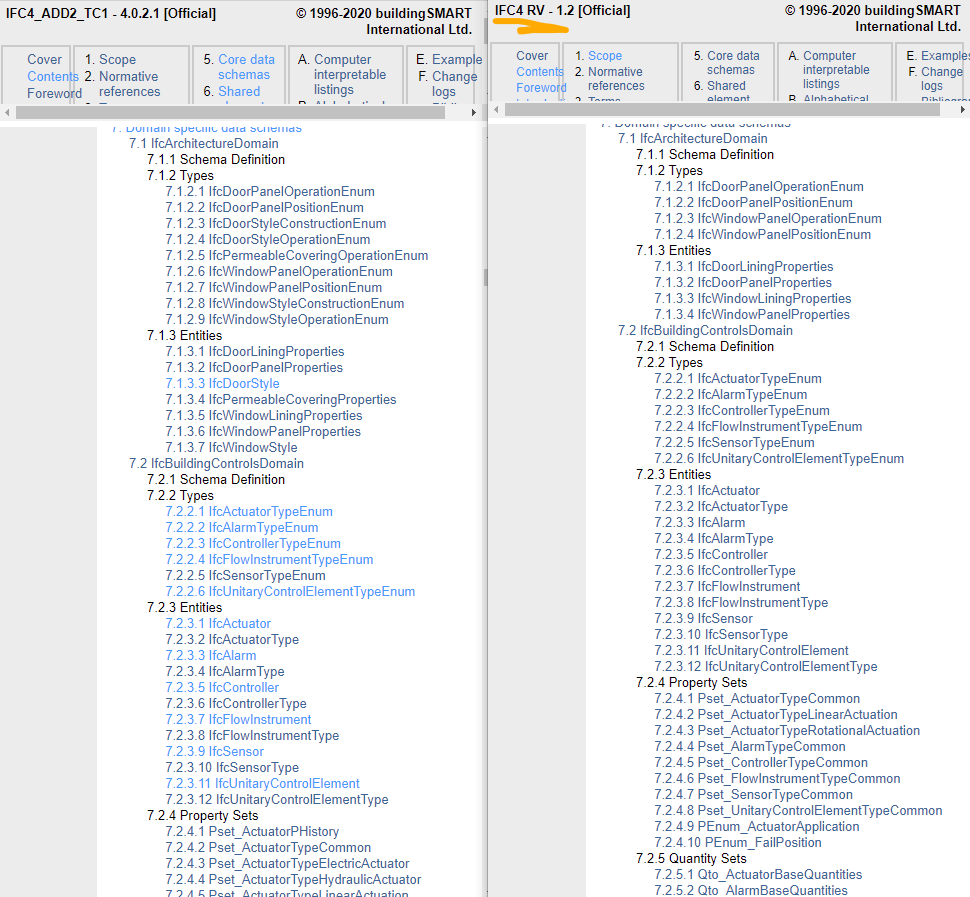
\includegraphics[width=0.9\textwidth]{MVD es un subconjunto del esquema IFC}

El concepto de MVD ha pasado desapercibido porque, en la práctica, casi siempre se suele utilizar la misma vista MVD:  `IFC 2x3 Coordination View (CV) 2.0'; pensada para compartir modelos entre disciplinas, en el dominio de edificación. \url{https://standards.buildingsmart.org/MVD/RELEASE/IFC2x3/TC1/CV2_0/IFC2x3_CV2_0.zip}

Esa MDV se definió en la versión 2x3 de IFC y como, en su momento, era la única MVD definida completamente, es la que utilizaron los principales fabricantes de software de modelado BIM para basar en ella sus módulos de exportación/importacón IFC.

Pero  existen también otras MVDs:
\begin{itemize}
\item Coordination View 2.0 2x3 Surface Geometry: pensada para visualización, coordinación de diseño y análisis de colisiones.
\item IFC 2x3 Basic FM Handover View: pensada para la gestión de activos.
\\ \url{https://technical.buildingsmart.org/wp-content/uploads/2021/01/GSC-001%20Basic%20HandOver%20to%20Facility%20Management.zip}
\item IFC4 Reference View (RV): la evolución de CV, y, como ella, bastante enfocada en la representación geométrica del modelo.
\\ \url{https://standards.buildingsmart.org/MVD/RELEASE/IFC4/ADD2_TC1/RV1_2/HTML/}
\item IFC4 Design Transfer View (DTV): una ampliación de RV para contemplar también la edición de elementos (mover, modificar, eliminar), con un alcance limitado predefinido.
\end{itemize}

Todas las MVDs definidas hasta ahora se pueden consultar en: \url{https://technical.buildingsmart.org/standards/ifc/mvd/mvd-database/}





\newpage
\section{Comprensión del esquema (I): Building Domain}

\subsection{Aspectos técnicos del esquema IFC}
El esquema IFC forma un sistema estandarizado para describir en forma digital un entorno de construcción, bien sea para construir edificios o para construir infraestructuras.

Para ello, definen y detallan:
\begin{itemize}
\item \textbf{Clases}: las ideas básicas que se intentan formalizar, entidades acerca de\ldots
\begin{itemize}
\item \ldots objetos físicos: los ``entes'' construibles.
\item \ldots conceptos abstractos: otros ``entes'' que de alguna manera participan o tienen relación con el proceso de construcción.
\end{itemize}
\item \textbf{Atributos}: propiedades intrínsecas que describen las entidades.
\item \textbf{Propiedades y cuantificadores}: propiedades extrínsecas que se pueden aplicar a las entidades, aportando información adicional sobre estas.
\item \textbf{Relaciones}: interacciones y enlaces entre entidades.
\end{itemize}

\vspace{0.3cm}
Hay varias versiones del esquema IFC, algunas retiradas, otras publicadas/oficiales, y otras de trabajo/construyendose:
\\ \url{https://technical.buildingsmart.org/standards/ifc/ifc-schema-specifications/}

A día de hoy (Mayo 2021) las dos versiones oficiales en activo son:
\begin{itemize}
\item IFC2x3 TC1, de 2005-2007: \begin{scriptsize}\url{https://standards.buildingsmart.org/IFC/RELEASE/IFC2x3/TC1/HTML/} \end{scriptsize}
\item IFC4 ADD2 TC1, de 2013-2017: \begin{scriptsize}\url{https://standards.buildingsmart.org/IFC/RELEASE/IFC4/ADD2_TC1/HTML/}\end{scriptsize}
\end{itemize}

\vspace{0.3cm}
Para facilitar su uso por parte de herramientas informatizadas. Las especificaciones del esquema IFC están disponibles en diversos formatos formales, directamente legibles por máquinas:
\begin{itemize}
\item EXPRESS: es un lenguaje para describir modelos dentro de un entorno de fabricación de producto; es parte del lenguaje STEP.
\\ \url{https://en.wikipedia.org/wiki/EXPRESS_%28data_modeling_language%29}
\\A día de hoy es el lenguaje oficial en que se trabajan las especificaciones IFC. 
\\Aunque, para la siguiente versión el trabajo se está realizando más bien en lenguaje UML (\url{https://en.wikipedia.org/wiki/Unified_Modeling_Language}), sobre un servidor compartido en EA (\url{https://sparxsystems.com/}) \footnote{\url{https://www.buildingsmart.org/wp-content/uploads/2020/06/IR-CS-WP2-UML_Model_Report_Part-1_.pdf}} 

\item XSD: es un lenguaje para describir estructuras internas de archivos XML según el tipo de información que vayan a contener.
\\ \url{https://en.wikipedia.org/wiki/XML_Schema_(W3C)} 
\\ \url{https://www.w3.org/standards/xml/schema.html}
\\ \url{https://www.w3.org/standards/xml/}

\item OWL: es un lenguaje para describir ontologias (vocabularios) para trabajar un determinado área de conocimiento ({\small \url{https://es.wikipedia.org/wiki/Ontolog%C3%ADa_(inform%C3%A1tica)}}.
\\ RDF y TTL: son lenguajes para escribir información en formato semántico.
\\ \url{https://en.wikipedia.org/wiki/Web_Ontology_Language}
\\ \url{https://en.wikipedia.org/wiki/RDF_Schema}
\\ \url{https://www.w3.org/standards/semanticweb/ontology}
\\ \url{https://www.w3.org/standards/semanticweb/data}
\\ \url{https://www.w3.org/standards/semanticweb/}
\\ \url{https://www.w3.org/TR/owl2-overview/}
\\ \url{https://www.w3.org/TR/rdf-schema/}
\end{itemize}

Por otro lado, los modelos IFC generados pueden ser escritos a un archivo en diversos formatos:
\begin{itemize}
\item STEP Pysical File (con extensión .ifc): a día de hoy, es la forma habitual de escribir un archivo IFC. 
\\ \url{https://en.wikipedia.org/wiki/ISO_10303-21}
\\ \url{https://www.une.org/encuentra-tu-norma/busca-tu-norma/iso/?c=063141}
\item STEP data in XML format (con extensión .ifcXML): es una forma alternativa de escribir un archivo IFC.
\\ \url{https://en.wikipedia.org/wiki/ISO_10303-28}
\\ \url{https://www.une.org/encuentra-tu-norma/busca-tu-norma/iso/?c=040646}
\item comprimido (con extensión .ifcZIP): al ser formatos textuales, tanto SPF como XML ven reducido muchísimo su tamaño de archivo cuando se comprimen.
\item web semántica:
\\ \url{https://en.wikipedia.org/wiki/Semantic_Web}
\\ \url{https://en.wikipedia.org/wiki/Resource_Description_Framework}
\\ \url{https://technical.buildingsmart.org/standards/ifc/ifc-formats/ifcowl/}
\begin{itemize}
\item TURTLE (.ttl): 
\\ \url{https://www.w3.org/TR/turtle/}
\item RDF/XML (.rdf):
\\\url{https://www.w3.org/TR/rdf-syntax-grammar/}
\end{itemize}
\item JSON, JavaScript Object Notation (.json): a día de hoy es un formato muy popular para intercambio de datos en el mundillo web; cada vez más lenguajes de programación tienen soporte directo para él. Se está barajando como futura alternativa para los archivos IFC.
\\ \url{https://www.json.org/json-en.html}
\item HDF, Hierachical Data Format (.hdf): es un formato binario de base de datos; produce archivos muy compactos; pero no legibles por humanos (no es textual). Se está barajando como una posible futura alternativa para escribir  archivos IFC.
\\ \url{https://en.wikipedia.org/wiki/Hierarchical_Data_Format}
\\ ISO 10303-26 {\tiny \url{https://www.une.org/encuentra-tu-norma/busca-tu-norma/iso/?c=050029}}
\end{itemize}

\subsection{Cómo se estructura el esquema IFC}

\subsubsection{Clases y atributos (información básica)}

El esquema IFC está definido ``con orientación a objetos'' (OO), en el sentido más o menos ``informático'' (OOP) de la frase . Es decir:
\begin{itemize}
\item Se definen \textit{clases} para representar cada entidad con las que se trabaja. Por ejemplo, la clase IfcDoor representa una puerta, IfcUnitaryControlElement un termostato, IfcBeam una viga, IfcBoiler una caldera, IfcTask una tarea, IfcCostItem un elemento de coste, etc.
\item Cada clase tiene una serie de atributos que recogen la información principal que define esa entidad. Por ejemplo, IfcUnitaryControlElement puede ser otros muchos elementos de control, pero lo que lo hace ser un termostato es poner el valor THERMOSTAT en su atributo PredefinedType. Por ejemplo, para indicar una puerta corredera que se desliza hacia la izquierda cuando se abre, hay que poner el valor SLIDING\_TO\_LEFT en el atributo OperationType de IfcDoor.

\item Se diferencia entre la definición genérica de una entidad $\rightarrow$ la clase. Y cada una de esas entidades concretas insertada dentro de un modelo $\rightarrow$ una \textit{instancia} (ejemplar) de la clase.

\item Unas clases pueden derivarse de otras, \textit{heredando} sus atributos. Esto se hace para evitar repetir atributos que son comunes a varias clases. Para ello se definen esas clases como hijas de una clase madre que contiene los atributos comunes que han de estar presentes en todas ellas.
\\Esta herencia se puede anidar tanto como sea necesario: madre - hija - nieta - bisnieta - \ldots. 
\\En concreto, el esquema IFC tiende a tener muchos niveles; por ejemplo: IfcDoor hereda de IfcBuildingElement, que a su vez hereda de IfcElement, que a su vez lo hace de IfcProduct, este de IfcObject, este de IfcObjectDefinition y , al final, de IfcRoot.
\\Este anidamiento múltiple puede resultar confuso, pero lo único que está indicando es que IfcDoor, además de los suyos propios, tiene también todos los atributos de IfcRoot, de IfcObjectDefinition, de IfcObject, de IfcProduct, de IfcElement y de IfcBuildingElement.
\end{itemize}

Las clases fundamentales del esquema IFC, de las que derivan casi todas las demás clases importantes son:
\begin{itemize}
\item IfcRoot: \url{https://standards.buildingsmart.org/IFC/RELEASE/IFC4/ADD2_TC1/HTML/link/ifcroot.htm}
\item IfcObjectDefinition: \url{https://standards.buildingsmart.org/IFC/RELEASE/IFC4/ADD2_TC1/HTML/link/ifcobjectdefinition.htm}
\item IfcPropertyDefinition: \url{https://standards.buildingsmart.org/IFC/RELEASE/IFC4/ADD2_TC1/HTML/link/ifcpropertydefinition.htm}
\item IfcRelationship: \url{https://standards.buildingsmart.org/IFC/RELEASE/IFC4/ADD2_TC1/HTML/link/ifcrelationship.htm}
\end{itemize}

Los atributos con la información básica de las entidades de cada clase pueden ser:
\begin{itemize}
\item Atributos Directos: datos propiamente dichos que se ponen a la entidad.

\item Atributos Inversos: datos redundantes, datos que ya están puestos como directos en algún atributo de alguna otra entidad del modelo.

Los atributos inversos tienen un doble propósito
\begin{itemize}
\item facilitar la navegación; permitiendo consultar qué está relacionado con qué, partiendo desde cualquier extremo de la relación; es decir, navegar en un sentido o en otro.
\item reforzar la integridad; de forma parecida a como la doble entrada lo hace en contabilidad.
\end{itemize}

Los atributos inversos suelen aparecer sobre todo en clases que representan relaciones. Toda relación se puede interpretar en uno o en otro sentido: por ejemplo, una ventana está situada sobre un hueco en un muro; pero, a su vez, el muro tiene un hueco sobre el que se sitúa una ventana.
\\ \url{https://standards.buildingsmart.org/IFC/RELEASE/IFC4/ADD2_TC1/HTML/annex/annex-e/wall-with-opening-and-window.htm}

\begin{footnotesize}
nota: En el ejemplo del enlace citado aparece una ventana (IfcWindow). Pero en el diagrama de detalle que he encontrado aparece una puerta (IfcDoor). A efectos prácticos de esta explicación, ambas son intercambiables (ambas derivan de IfcElement). 

\end{footnotesize}
Un muro (IfcWall) y un hueco (IfcOpeningElement) están relacionados con la relación IfcRelVoidsElement.
\\El hueco y una puerta (IfcDoor) están relacionados con la relación IfcRelFillsElement.

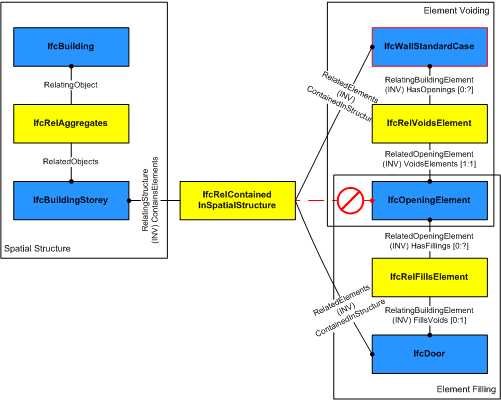
\includegraphics[width=\textwidth]{ifcrelfillselements-fig1}
\begin{footnotesize}
\\ \url{https://standards.buildingsmart.org/IFC/RELEASE/IFC4/ADD2_TC1/HTML/link/ifcelement.htm}
\\ \url{https://standards.buildingsmart.org/IFC/RELEASE/IFC4/ADD2_TC1/HTML/link/ifcopeningelement.htm}
\\ \url{https://standards.buildingsmart.org/IFC/RELEASE/IFC4/ADD2_TC1/HTML/link/ifcrelvoidselement.htm}
\\ \url{https://standards.buildingsmart.org/IFC/RELEASE/IFC4/ADD2_TC1/HTML/link/ifcrelfillselement.htm}
\end{footnotesize}

La relación IfcRelVoidsElement tiene un atributo directo, RelatingBuildingElement, que admite valores de tipo IfcElement (la clase muro, IfcWall, deriva de la clase IfcElement). Pero, a su vez, el muro tiene un atributo inverso, HasOpenings, que admite valores de tipo IfcRelVoidsElement.
\vspace{0.1cm}
\\ 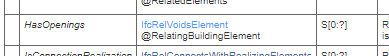
\includegraphics[scale=0.8]{atributo HasOpenings}
\vspace{0.1cm}
\\ 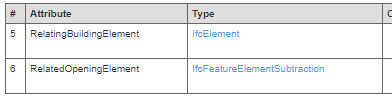
\includegraphics[scale=0.8]{atributos de IfcRelVoidsElement}
\\ 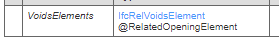
\includegraphics[scale=0.8]{atributo VoidsElements}
\\La relación IfcRelVoidsElement tiene otro atributo directo, RelatedOpeningElement, que admite valores de tipo IfcFeatureElementSubtraction (la clase hueco, IfcOpeningElement, deriva de la clase IfcFeatureElementSubstraction). Pero, a su vez, el hueco tiene un atributo inverso, VoidsElements, que admite valores de tipo IfcRelVoidsElement.

Como se ve en el gráfico, el hueco y la puerta siguen un esquema similar. Solo que con la relación IfcRelFillsElement y los atributos inversos HasFillings y FilsVoids, respectivamente.

\end{itemize}



\subsubsection{IfcRoot, la clase de la que derivan casi todas las demás clases}
IfcRoot es la clase raíz, una clase de la que derivan muchísimas otras clases. Aporta a todas ellas los atributos:
\begin{itemize}
\item GlobalID: un identificador único. Basado en GUID (\url{https://en.wikipedia.org/wiki/Universally_unique_identifier}), pero con algunas limitaciones respecto a este (\url{https://standards.buildingsmart.org/IFC/RELEASE/IFC4/ADD2_TC1/HTML/link/ifcgloballyuniqueid.htm}).
\item OwnerHistory: información acerca de quien ha generado el objeto (usualmente suele rellenarse con el nombre del sofware de modelado que exporta el IFC) y cuándo ha sido modificado por última vez. 
\item Name: un nombre corto, limitado a 256 caracteres.
\item Description: un nombre largo.
\end{itemize}

\subsubsection{IfcObject, la clase de las que derivan las clases ``tangibles''}
De la clase IfcObject derivan:
\begin{itemize}
\item \textbf{IfcProduct}: representa cosas físicas que se incorporan al edificio o infraestructura. Aporta a sus clases derivadas, entre otros,
\begin{itemize}
\item el atributo ObjectPlacement (para indicar una ubicación)
\item y el atributo Representation (para indicar una representación geométrica)
\end{itemize}

\item \textbf{IfcProcess}: representa una actividad o un evento.

\item \textbf{IfcResource}: representa algo utilizado o consumido durante el proceso de construcción.

\item \textbf{IfcControl}: representa algo que modula, limita o regula de algún modo el uso de un producto, proceso o recurso.

\item \textbf{IfcActor}: representa organizaciones (empresas) o personas (individuos).

\item \textbf{IfcProject}: es el ``contenedor'' principal de todo lo demás que está dentro de un determinado modelo IFC. Solo puede haber una única instancia de la clase IfcProject en cada archivo IFC.
\\Aviso: al estar derivado de IfcRoot, cada instancia de IfcProject tiene su GlobalID único; lo que puede dar lugar a problemas al federar diversos archivos IFC, ya que cada uno de ellos tiene un GlobalID distinto $\rightarrow$ representa un ``proyecto'' distinto. 
\\Nota: otros ``contenedores'' para organizar las distintas partes de un modelo pueden ser las clases IfcSite (emplazamiento), IfcBuilding (edificio), IfcBuildingStorey (planta), \ldots; de estas si que puede haber tantas instancias de cada clase como se necesiten dentro de un mismo archivo IFC. 

\item \textbf{IfcGroup}: representa agrupaciones lógicas de entidades. Una misma entidad puede pertenecer a varios grupos. Un grupo puede estar dentro de otros grupos. Es una clase muy útil, pero poco utilizada (¿quizá porque Revit no tiene ningún soporte para ella?)
\end{itemize}

\newpage
\subsubsection{Conjuntos de Propiedades (cómo se inserta información)}
Los conjuntos de propiedades recogen información que se puede asignar de forma libre a los objetos del modelo. \url{https://standards.buildingsmart.org/IFC/RELEASE/IFC4/ADD2_TC1/HTML/link/ifcpropertydefinition.htm}

Los conjuntos de propiedades se asocian a los objetos a través del atributo `IsDefinedBy' de IfcObject, que indica relaciones de la clase `IfcRelDefinesByProperties' \url{https://standards.buildingsmart.org/IFC/RELEASE/IFC4/ADD2_TC1/HTML/link/ifcreldefinesbyproperties.htm}. 

$IsDefinedBy \rightarrow RelatedObjects / RelatingPropertyDefinition \rightarrow DefinesOcurrence / HasProperties$
\\ 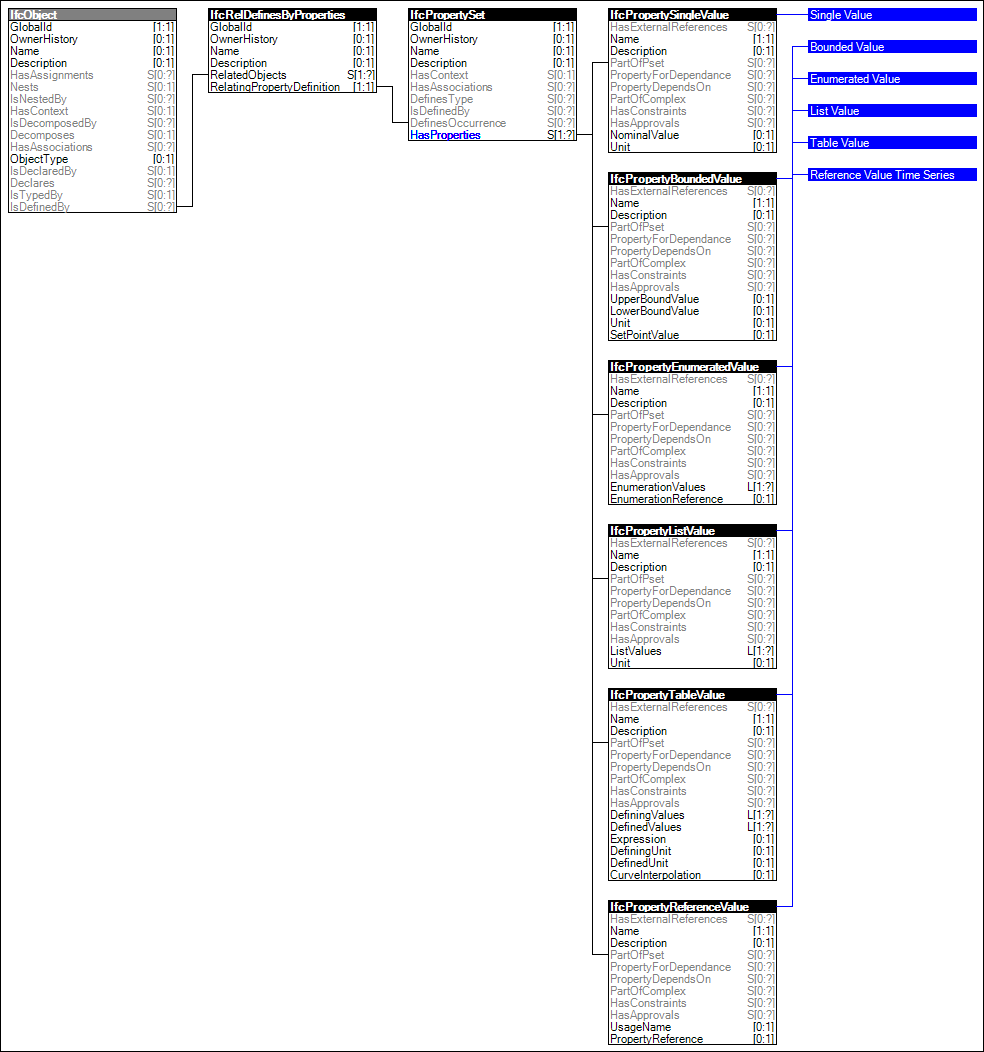
\includegraphics[width=\textwidth]{property-sets-for-objects}
\\ \url{https://standards.buildingsmart.org/IFC/RELEASE/IFC4/ADD2_TC1/HTML/link/property-sets-for-objects.htm}

\newpage
$IsDefinedBy \rightarrow RelatedObjects / RelatingPropertyDefinition \rightarrow DefinesOcurrence / Quantities$
\\ 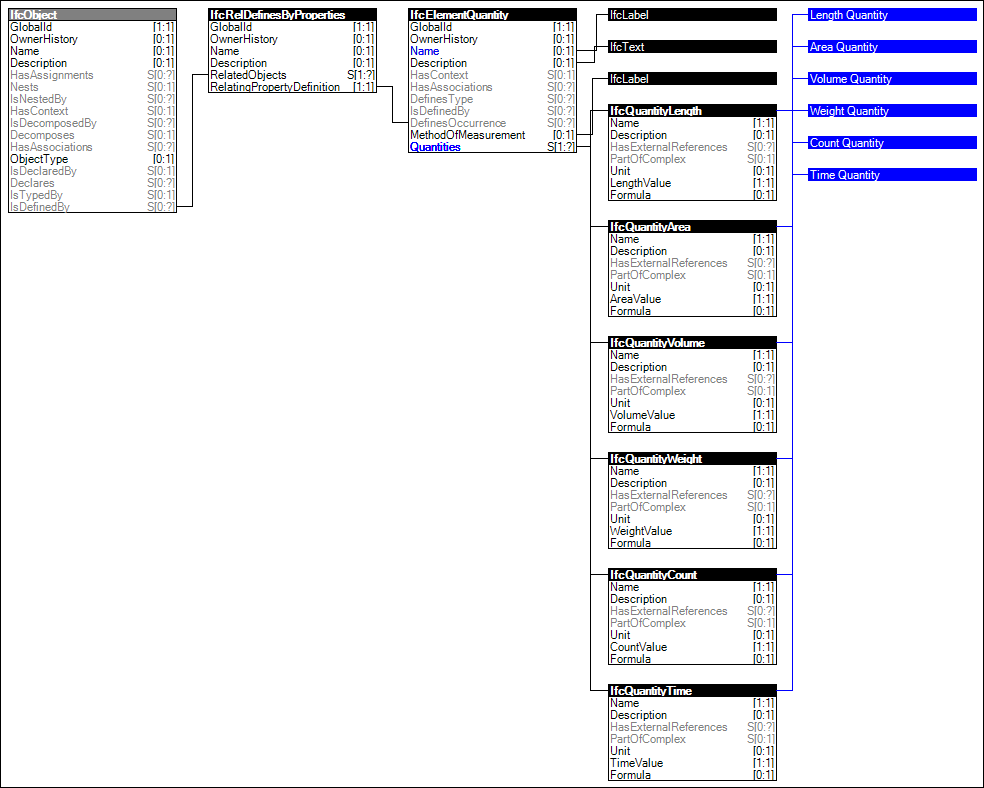
\includegraphics[width=\textwidth]{quantity-sets}
\\ \url{https://standards.buildingsmart.org/IFC/RELEASE/IFC4/ADD2_TC1/HTML/link/quantity-sets.htm}


\vspace{0.5cm}
Los conjuntos de propiedades pueden ser:
\begin{itemize}
\item Estandares, definidos en el propio esquema IFC. Sus nombres suelen comenzar por \textbf{PSet\_} o por \textbf{Qto\_} según contengan información general o relativa a mediciones, respectivamente.
\item Personalizadas, introducidas por el software de modelado utilizado para confeccionar el modelo nativo que se ha exportado a IFC.
\item Personalizadas, introducidas por nosotros mismos al modelar.
\end{itemize}
Aviso: es importante evitar que los nombres de los conjuntos de propiedades personalizados comiencen por PSet\_ o por Qto\_; para evitar confundirlos con los estandares. 

\vspace{0.5cm}
\begin{small}\url{https://standards.buildingsmart.org/IFC/RELEASE/IFC4/ADD2_TC1/HTML/link/ifcproperty.htm}\end{small}

Cada propiedad puede contener:
\begin{itemize}

\item Valores concretos: IfcSimpleProperty
\\ \begin{footnotesize} \url{https://standards.buildingsmart.org/IFC/RELEASE/IFC4/ADD2_TC1/HTML/link/ifcsimpleproperty.htm}\end{footnotesize}
\\que pueden ser:
\begin{itemize}
\item Single Value: un valor libre
\item Bounded Value: un valor limitado entre un mínimo y un máximo.
\item Enumerated Value: un valor a elegir de entre unos predeterminados.
\item List Value: múltiples valores, organizados en forma de lista.
\item Table Value: múltiples valores, organizados en forma de tabla.
\end{itemize}

\item Valores compuestos: IfcComplexProperty
\\ \begin{footnotesize} \url{https://standards.buildingsmart.org/IFC/RELEASE/IFC4/ADD2_TC1/HTML/link/ifccomplexproperty.htm}\end{footnotesize}
\\son propiedades que contienen otros conjuntos de propiedades, en una estructura arbórea.

\end{itemize}

\vspace{0.5cm}
Los valores concretos pueden ser a su vez:
\begin{itemize}
\item Básicos (solo valor): IfcSimpleValue
\\ \url{https://standards.buildingsmart.org/IFC/RELEASE/IFC4/ADD2_TC1/HTML/link/ifcsimplevalue.htm}
\item Magnitudes (valor + unidad de medida): IfcMeasureValue
\\ \url{https://standards.buildingsmart.org/IFC/RELEASE/IFC4/ADD2_TC1/HTML/link/ifcmeasurevalue.htm}
\item Magnitudes derivadas: IfcDerivedMeasureValue
\\ \url{https://standards.buildingsmart.org/IFC/RELEASE/IFC4/ADD2_TC1/HTML/link/ifcderivedmeasurevalue.htm} 
\end{itemize}

\newpage
\subsubsection{Relaciones entre entidades (cómo se arma el modelo IFC y toda la información que contiene)}
De la clase IfcRelationship derivan:
\begin{itemize}
\item IfcRelAssigns y sus derivadas, como por ejemplo IfcRelAssignsToProcess o IfcRelAssignsToActor o IfcRelAssignsToResource.

\item IfcRelAssociates y sus derivadas, como por ejemplo IfcRelAssociatesDocument o IfcRelAssociatesMaterial.

\item IfcRelConnects y sus derivadas, como por ejemplo IfcRelContainedInSpatialStructure que define relaciones de pertenencia a un determinado ``contenedor'' espacial.

\item IfcRelDeclares.

\item IfcRelDecomposes y sus derivadas, como por ejemplo IfcRelAggregates que define relaciones de jerarquia de anidamiento espacial entre ``contenedores'' o IfcRelNests que define relaciones de anidamiento entre una entidad compuesta y sus partes constituyentes.

\item IfcRelDefines y sus derivadas, como por ejemplo IfcRelDefinesByProperties.
\end{itemize}

\vspace{0.5cm}
Por ejemplo, las relaciones entre estructuras espaciales suelen ser de esta forma:
\vspace{0.3cm}
\\ 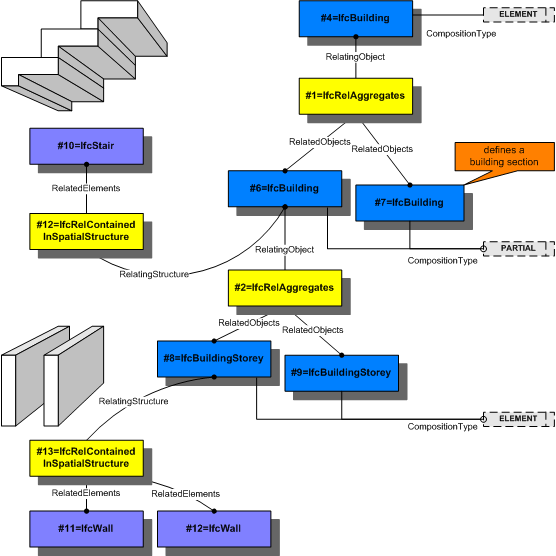
\includegraphics[width=\textwidth]{ifcrelcontainedinspatialstructure-fig1}

\subsection{Unas notas sobre clasificación de entidades}
Uno de los requisitos básicos para que sea posible una colaboración fluida entre los diversos actores en un proyecto de construcción: todos nos hemos de referir de igual manera a cada elemento del proyecto.

Por otro lado, para garantizar la interoperabilidad de las diversas búsquedas, listados, informes, presupuestos, comunicaciones,\ldots es imprescindible utilizar un sistema común de identificación y agrupación de los elementos.

Es decir, es importante cuidar la coherencia de toda la información que se va elaborando.
\\Vale cualquier cosa que se acuerde entre los participantes.
\\Mejor si es consistente con alguno de los  estandares existentes.
\\Pero lo realmente importante es que se mantenga coherente durante todo el ciclo de vida del proyecto, para todos los participantes en el mismo. 

\vspace{0.5cm}
En el esquema IFC, las entidades presentes en el modelo se pueden clasificar por tres vías:

\subsubsection{Por sub-tipado de clase}
La propia clase que asignamos a una entidad es la que nos indica qué entidad es. 

Un par de ejemplos:

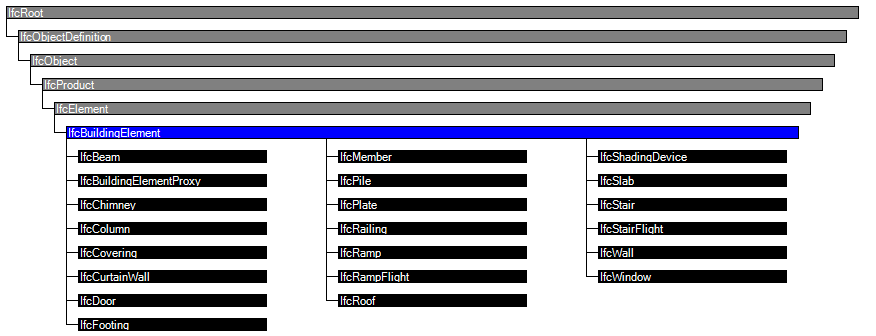
\includegraphics[width=0.7\textwidth]{ifcbuildingelement}

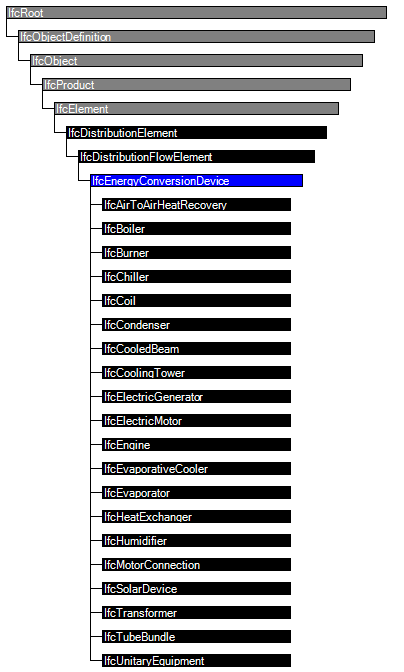
\includegraphics[scale=0.6]{ifcenergyconversiondevice}

\subsubsection{Por enumeración de tipo}
El valor que pongamos en el atributo PredefinedType de una entidad nos precisa qué entidad es.
\\ 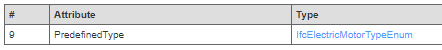
\includegraphics[scale=1.1]{atributo PredefinedType para un IfcElectricMotor} 
\\ 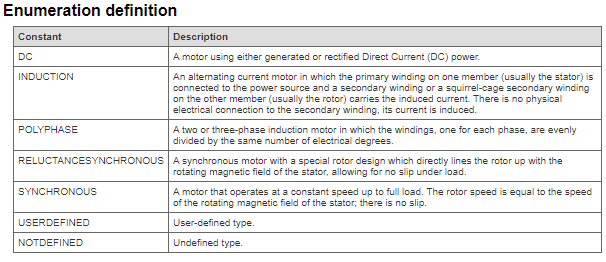
\includegraphics[scale=1]{enumeracion IfcElectricMotorTypeEnum}

nota: si se indica USERDEFINED, se debe indicar el tipo en el atributo ObjectType de la entidad (atributo heredado de IfcObject).
\\ 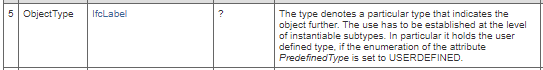
\includegraphics[scale=1]{atributo ObjectType}

\subsubsection{Por referencia a un sistema de clasificación externo}
Utilizando la relación IfcRelAssociatesClassification, podemos relacionar una entidad con un código dentro de un determinado sistema de clasificación: IfcClassification o IfcClassificationReference.

\begin{footnotesize}
\url{https://standards.buildingsmart.org/IFC/RELEASE/IFC4/ADD2_TC1/HTML/link/ifcclassification.htm}
\\ \url{https://standards.buildingsmart.org/IFC/RELEASE/IFC4/ADD2_TC1/HTML/link/ifcclassificationreference.htm}
\\ \url{https://standards.buildingsmart.org/IFC/RELEASE/IFC4/ADD2_TC1/HTML/link/ifcrelassociatesclassification.htm}
\end{footnotesize}

En el mundo hay multitud de sistemas de clasificación. Por ejemplo:
\begin{itemize}

\item GuBIMclass: se utiliza en Cataluña.
\\ \url{https://gubimclass.org/es/}

\item Ommiclass: se utiliza en UK
\\ \url{https://www.csiresources.org/standards/omniclass/standards-omniclass-about}

\item MasterFormat: se utiliza en USA.
\\ \url{https://www.csiresources.org/standards/masterformat}

\item UniFormat: se utiliza en USA.
\\ \url{https://www.thenbs.com/our-tools/uniclass-2015#classificationtables}
\\ \url{https://www.csiresources.org/standards/uniformat}

\item NL SfB:  se utiliza en Holanda.
\\ \url{https://www.bimloket.nl/p/107/NL-SfB}

\item UNI 11337: se utiliza en Italia.
\\ \url{http://store.uni.com/catalogo/uni-ts-11337-3-2015/}

\item DIN SPEC 91400: se utiliza en Alemania 
\\ \url{https://www.din.de/de/mitwirken/normenausschuesse/nabau/veroeffentlichungen/wdc-beuth:din21:267208318}

\item NS 3451: se utiliza en Noruega
\\ \url{https://www.standard.no/fagomrader/bygg-anlegg-og-eiendom/ns-3420-/ns-3450----ns-3451---ns-3459-2/}

\item CoClass: se utiliza en Suecia
\\ \url{https://coclass.byggtjanst.se/}

\item Talo2000: se utiliza en Finlandia
\\ \url{https://www.rakennustieto.fi/index/tuotteet/nimikkeistot_21/talo2000.html}

\item CCS: se utiliza en Dinamarca
\\ \url{https://molio.dk/produkter/digitale-vaerktojer/gratis-vaerktojer/ccs-cuneco-classification-system}

\end{itemize}
\url{https://buildingsmart.fi/wp-content/uploads/2019/12/20191021-Nordic-Study-S2_FINAL.pdf}

nota: Dion Moult tiene un resumen técnico muy bueno de los principales sistemas de clasificación empleados en el mundo. Con relaciones detalladas de cada uno de ellos en formato IFC (STEP) y XML  \url{https://github.com/Moult/IfcClassification}


\vspace{1cm}
Aviso:
\\Una cosa son las posibilidades del esquema IFC y otra cosa lo que cada fabricante haya querido implementar en el software de autoria con el que modelamos. Como botón de muestra, un artículo acerca del atributo PredefinedType de IFC visto desde el software de modelado Revit: \url{https://bimblog.bondbryan.co.uk/ifc-industry-foundation-classes-predefined-types-in-autodesk-revit/}



\subsection{Unas notas sobre representación geométrica}
La representación geométrica está contemplada como un aspecto más dentro de la información que puede darse sobre cada entidad presente en un modelo IFC. 

Aquellas entidades susceptibles de tener una ``presencia física'' (las derivadas de IfcProduct), contemplan su representación geométrica como una más de las múltiples informaciones que se pueden registrar acerca de las mismas. 

La representación geométrica se suele indicar en el atributo Representation de la clase IfcProduct. Y este atributo suele contener entidades de la clase IfcProductRepresentation (\url{https://standards.buildingsmart.org/IFC/RELEASE/IFC4/ADD2_TC1/HTML/link/product-geometric-representation.htm}).

En IFC, hay diversas maneras de representar gráficamente un objeto:
\begin{itemize}
\item Con una ``caja'' que muestra sus límites externos, (Bounding Box).

\item Con curvas.

\item Con superficies.

\item Con cuerpos sólidos, bien sean:
\begin{itemize}
\item definidos de forma explícita, basados en superficies (IfcManifoldSolidBrep \url{https://standards.buildingsmart.org/IFC/RELEASE/IFC4/ADD2_TC1/HTML/link/ifcmanifoldsolidbrep.htm})
\item definidos de forma implícita, basados en barridos (IfcSweptAreaSolid \url{https://standards.buildingsmart.org/IFC/RELEASE/IFC4/ADD2_TC1/HTML/link/ifcsweptareasolid.htm}) o basados en extrusiones y operaciones booleanas (IfcCsgSolid \url{https://standards.buildingsmart.org/IFC/RELEASE/IFC4/ADD2_TC1/HTML/link/ifccsgsolid.htm}) 
\end{itemize}

\item IFC4 incorpora, además, representaciones basadas en splines. Mucho más precisas a la hora de representar geometrias complejas.
\\(IfcBSplineCurve \url{https://standards.buildingsmart.org/IFC/RELEASE/IFC4/ADD2_TC1/HTML/link/ifcbsplinecurve.htm}) 
\\(IfcBSplineSurface \url{https://standards.buildingsmart.org/IFC/RELEASE/IFC4/ADD2_TC1/HTML/link/ifcbsplinesurface.htm})
\end{itemize}   

Aviso:
\\No perder de vista que aquí también tenemos por un lado las capacidades de representación geométrica contempladas en el estandar IFC y por otro las capacidades gráficas del software nativo de modelado que se esté utilizando (por ejemplo: \url{https://www.plm.automation.siemens.com/global/en/products/plm-components/parasolid.html}).
\\Unas y otras capacidades pueden ser similares o pueden diferir bastante, siendo muy posible que se pierda definición geométrica en las conversiones. Entre otras razones, esta es una por la que se recomienda no utilizar IFC como herramienta de intercambio bidireccional entre distintos softwares de modelado.


\topskip0pt
\vspace*{\fill}
Más apuntes relativos al esquema IFC y sus especificaciones técnicas: \url{https://www.susosise.es/documentos/El_estandar_IFC.pdf}
\vspace*{\fill}
%
\newpage





\section{Comprensión del esquema (II): Infrastructure Domains, hasta IFC 4.3 RC3}


\subsection{¿Cómo desarrolla buildingSMART sus estandares?}

buildingSMART se organiza en una serie de estructuras internacionales:
\begin{itemize}
\item Comités: SC, SCE (executive) y SCTE (technical). Deciden y votan el paso de estado (propuesta - candidata - oficial) de las diversas versiones que se van elaborando de los distintos estandares.
\\ \url{https://www.buildingsmart.org/standards/organisation/}
\item Rooms (``habitaciones''): comités especialistas en determinados temas o dominios. Hacen de filtro y marcan  directrices para los distintos grupos de trabajo que van elaborando los estandares.
\\ \url{https://www.buildingsmart.org/standards/rooms/}
\end{itemize}
Y una serie de capítulos nacionales: \url{https://www.buildingsmart.org/chapter-directory/}.
\vspace{1cm}

A grandes rasgos, la elaboración de cualquier nueva versión de un estandar existente o de un nuevo estandar:
\begin{enumerate}
\item Comienza recopilando las necesidades de la industria.

\item En los Rooms y en los Grupos de Trabajo que se vayan formando, se van analizando esas necesidades y elaborando las especificaciones de lo que se necesita para satisfacerlas. De ahí sale una \textit{propuesta}.

\item Tras las pertinentes votaciones en los Comités, en caso de resultar aprobada la propuesta, se establecen distintos Proyectos para trabajar los diversos aspectos de la misma:
\begin{itemize}
\item Realizando implementaciones de prueba y simulaciones de trabajo.
\item Decidiendo los detalles de cada aspecto, hasta alcanzar amplios consensos en todos ellos.
\item Definiendo y elaborando detallados marcos de prueba de software para cada aspecto.
\end{itemize} 
De aquí surgen \textit{borradores de trabajo} y, tras las pertinentes votaciones en los Comités, se van proponiendo versiones \textit{candidatas}.

\item Cuando alguna de esas versiones candidatas está suficientemente madura. Con el visto bueno de los Rooms y tras las pertinentes votaciones en los Comités. Se emite una versión \textit{oficial}:
\begin{itemize}
\item Los distintos fabricantes de software comienzan a implantarla en sus productos.
\item Los usuarios comienzan a utilizarla.
\item Se comienzan los trabajos para elevarla a la categoría de norma ISO
\end{itemize}
\end{enumerate}

\vspace{1cm}
Algunos de los desarrollos que están en curso: \url{https://www.buildingsmart.org/standards/calls-for-participation/}

\subsection{Los nuevos dominios de infraestructura que se incorporarán en la futura versión 4.3 ¿o será 5?}

Hasta la versión 4, el esquema IFC se ha ido desarrollando pensando principalmente en el dominio de edificación.

Para incorporar los diversos dominios de infraestructuras, han sido necesarios una serie de ajustes de calado dentro de algunas clases del núcleo:
\begin{itemize}
\item Las clases ``contenedoras'' derivadas de IfcSpatialStructureElement ven modificada su jerarquia de derivación, introduciendose dos nuevas clases: \textbf{IfcFacility} e \textbf{IfcFacilityPart}. Se permite así acomodar nuevas clases junto a la que ya existian de IfcBuilding - IfcBuildingStorey. Se van incorporando: \textit{IfcBridge} - IfcBridgePart, \textit{IfcMarineFacility}, \textit{IfcRailway}, \textit{IfcRoad},\ldots
\begin{footnotesize}
\\ \url{https://standards.buildingsmart.org/IFC/DEV/IFC4_3/RC2/HTML/link/ifcspatialstructureelement.htm}
\\ \url{https://standards.buildingsmart.org/IFC/DEV/IFC4_3/RC2/HTML/link/ifcfacility.htm}
\\ \url{https://standards.buildingsmart.org/IFC/DEV/IFC4_3/RC2/HTML/link/ifcfacilitypart.htm}
\end{footnotesize}

\item IfcBuildingElement pasa a ser \textbf{IfcBuiltElement}, para acomodar nuevos elementos construibles que se pueden incorporar a las construcciones.
\begin{footnotesize}
\\ \url{https://standards.buildingsmart.org/IFC/DEV/IFC4_3/RC2/HTML/link/ifcbuiltelement.htm}
\end{footnotesize}

\item Se incorpora \textbf{IfcGeotechicalElement} y las clases necesarias para acomodar entidades relacionadas con los estudios geotécnicos y con los movimientos de tierras.
\begin{footnotesize}
\\ \url{https://standards.buildingsmart.org/IFC/DEV/IFC4_3/RC2/HTML/link/ifcgeotechnicalelement.htm}
\end{footnotesize}

\item Se incorpora \textbf{IfcAligment} y las clases necesarias para acomodar entidades relacionadas con el trazado de infraestructuras lineales, tales como carreteras y vías de ferrocarril.
\begin{footnotesize}
\\ \url{https://standards.buildingsmart.org/IFC/DEV/IFC4_3/RC2/HTML/link/ifcalignment.htm}

\end{footnotesize}
\end{itemize} 

Con motivo de estos cambios realizados en su núcleo. La futura nueva versión del esquema IFC (4.3 , ¿5?) no será retrocompatible con las versiones 2x3 y 4 actualmente vigentes. 


\newpage
\section{Comprensión (III) a través de los recursos web de bSI}

\subsection{Repaso general a la web y a los recursos presentes en ella}

Merece la pena dedicar un tiempo a navegar por la web de buildingSMART International:
\\ \url{https://www.buildingsmart.org/}
\\Y sus diversos capítulos nacionales, \url{https://www.buildingsmart.org/chapter-directory/}; 
\\como por ejemplo el español: \url{https://www.buildingsmart.es/}

\vspace{0.5cm}
Hay bastantes apartados interesantes:
\begin{itemize}

\item Sobre la propia organización interna y funcionamiento del organismo:
\\ 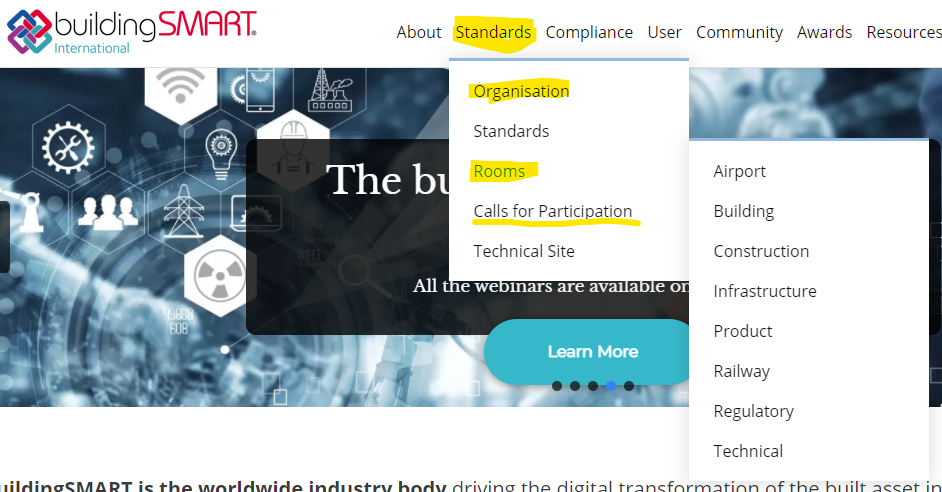
\includegraphics[width=0.8\textwidth]{web - Estandards - Organization - Rooms}
\\ 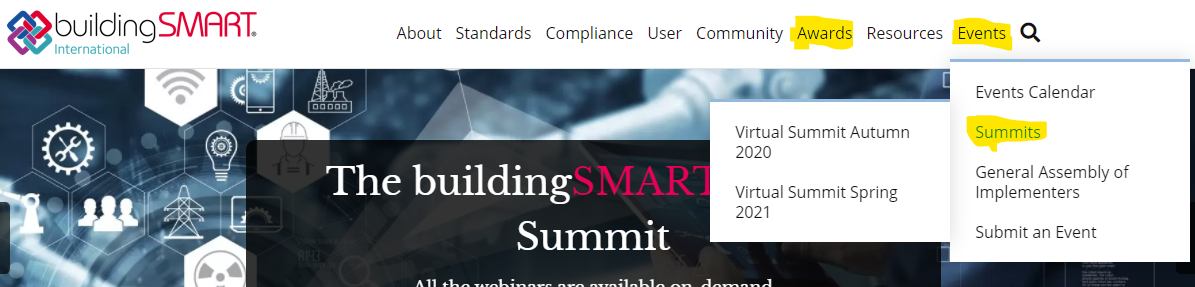
\includegraphics[width=\textwidth]{web - Events- Summits}
\begin{flushright}nota: videos en \url{https://vimeo.com/user94789481}\end{flushright}

\item Sobre aspectos técnicos:
\\ 
\includegraphics[width=\textwidth]{web - Standards - Technical Site}
\\ \url{https://technical.buildingsmart.org/}
\\ 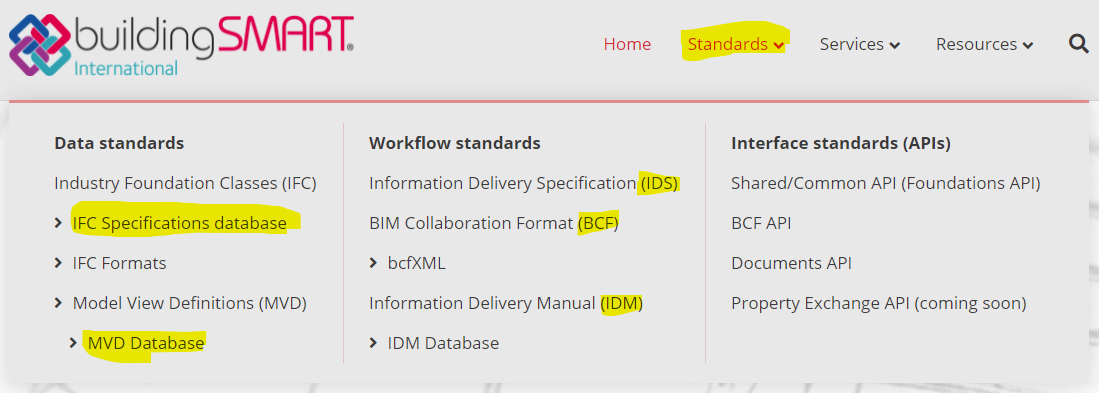
\includegraphics[width=\textwidth]{web - technical - Standards}
\\ 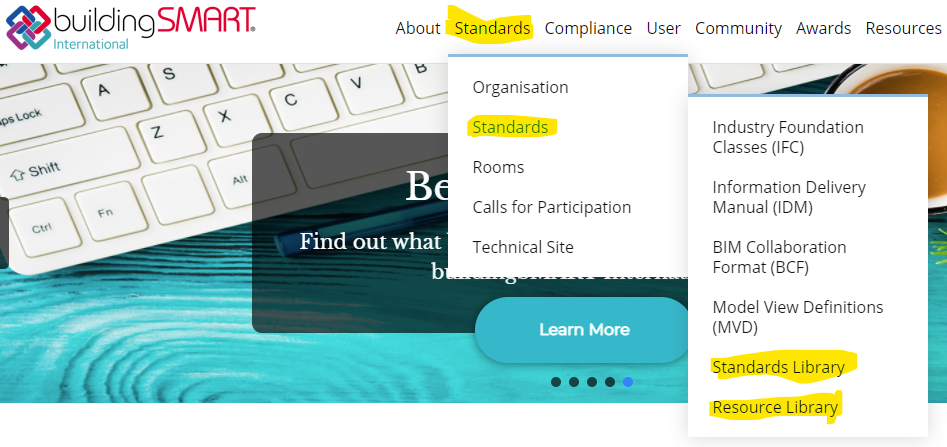
\includegraphics[width=0.7\textwidth]{web - Standards - Standards - libraries}

\item Sobre la comunidad de usuarios:
\\ 
\includegraphics[width=\textwidth]{web - User}
\\ \url{https://www.buildingsmart.org/users/forum/}
\\nota: El foro es muy activo y suele tener debates interesantes. Es un buen recurso para estar al día y aprender  cómo van gestándose los estandares. Además proporciona una visión acerca de las distintas formas de considerar los distintos conceptos en distintas partes del mundo y a través de los ojos de diversas disciplinas. Merece la pena hacerse miembro del mismo.
\\nota: Las guias de usuario colgadas en la web no son muchas por ahora. La idea es ir nutriendo este apartado con las guías que vayan escribiendo y aportando los participantes en la comunidad.

\item Sobre los servicios:
\\ 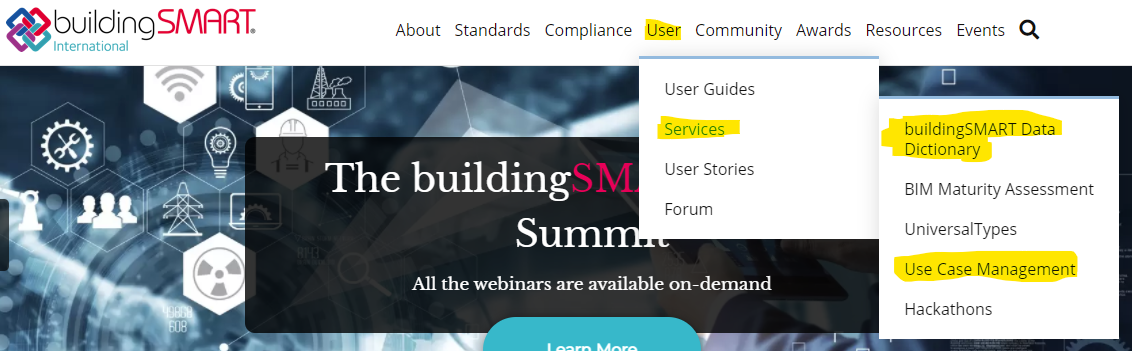
\includegraphics[width=0.8\textwidth]{web - User - Services}
\\ \url{https://technical.buildingsmart.org/}
\\ 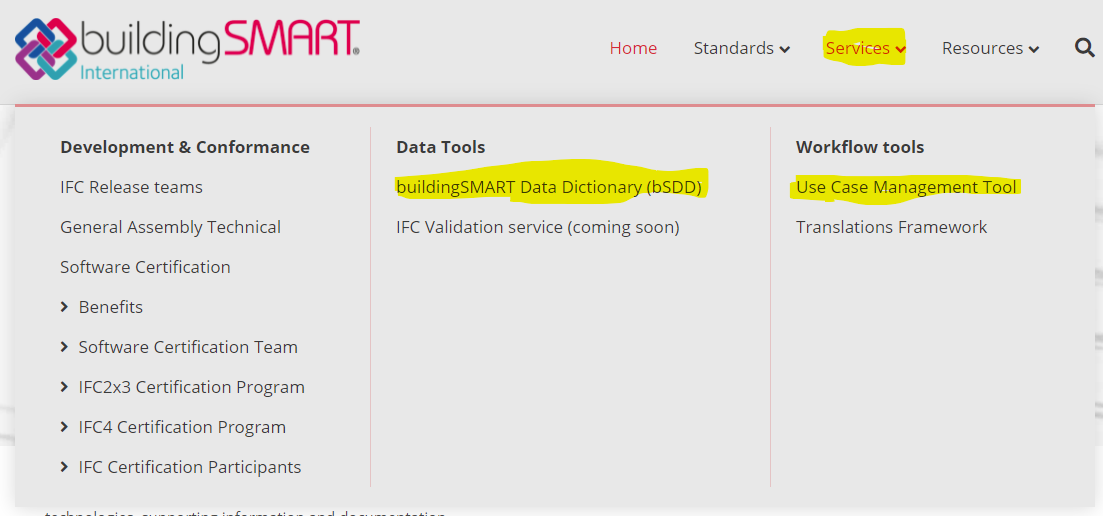
\includegraphics[width=\textwidth]{web - technical - Services}

nota: Los estandares técnicos de buildingSMART, hasta hace poco, estaban pensados para ser utilizados en base a intercambios de archivos.
\\En estos momentos están evolucionando para ser utilizados a base de servicios web, en plataformas ``cloud'', en la nube.

\item Sobre el desarrollo de los estandares y de utilidades auxiliares en torno a ellos:
\\ \url{https://github.com/buildingSMART}
\\ 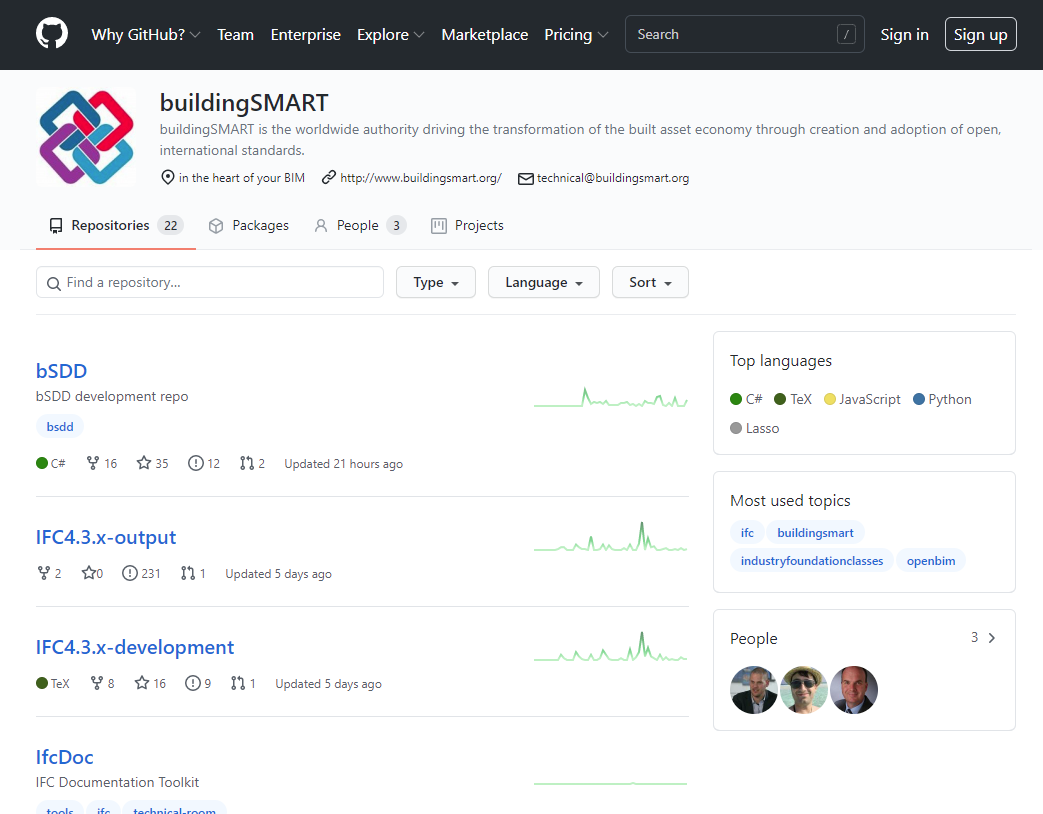
\includegraphics[width=\textwidth]{GitHub - pagina principal de buildingSMART}

\end{itemize}



\subsection{Repaso general a la estructura de la documentación técnica del esquema IFC}

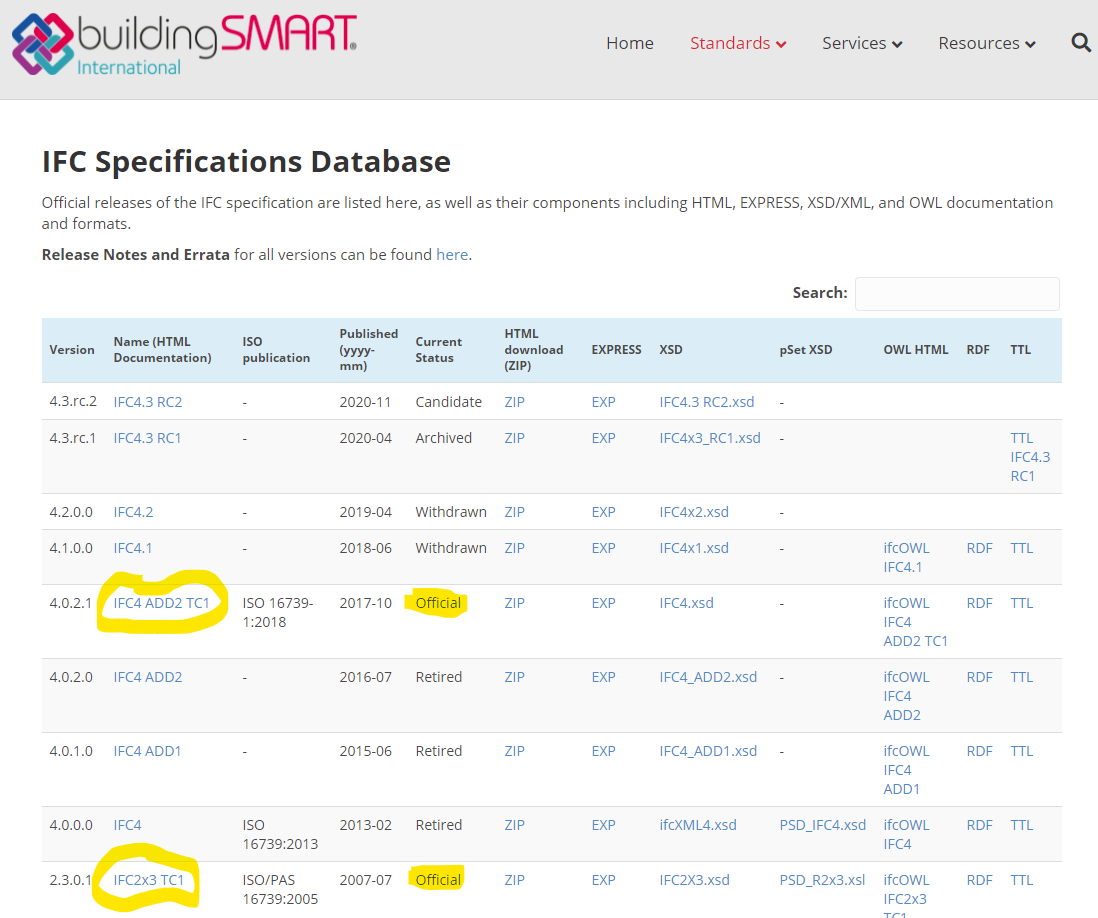
\includegraphics[width=0.95\textwidth]{web - IFC SpecificationsDatabase}

\url{https://technical.buildingsmart.org/standards/ifc/ifc-schema-specifications/}

notas: 
\\Los enlaces bajo la columna `Name (HTML Documentation)' nos llevan a las páginas web de las respectivas especificaciones, para permitir su lectura por parte de personas humanas.
\\Los enlaces bajo las columnas `EXPRESS', `XSD', 'pSet XSD', `OWL HTML', `RDF' y `TTL' permiten descargar archivos con las especificaciones expresadas en diversos lenguajes informáticos, para permitir su utilización por parte de softwares.


\subsubsection{Especificaciones del esquema IFC en su versión 4 (IFC4 ADD2 TC1)}

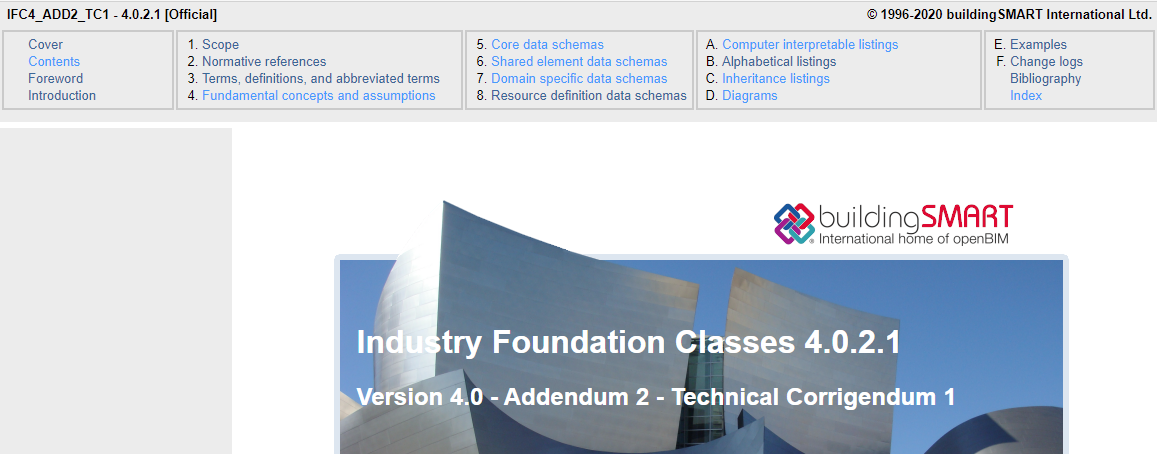
\includegraphics[width=\textwidth]{IFC4 - Portada}

\url{https://standards.buildingsmart.org/IFC/RELEASE/IFC4/ADD2_TC1/HTML/}

\textbf{Algunos trucos para navegar por la documentación:}

\begin{itemize}

\item Cualquier texto en azul y prácticamente cualquier cuadro en cualquier diagrama: son enlaces que nos llevan a la página correspondiente de la entidad citada en ellos.

\item La columna de la izquierda es muy importante. Nos muestra en todo momento ``la vecindad'' (otras entidades similares o relacionadas) de la entidad cuya página estamos viendo.

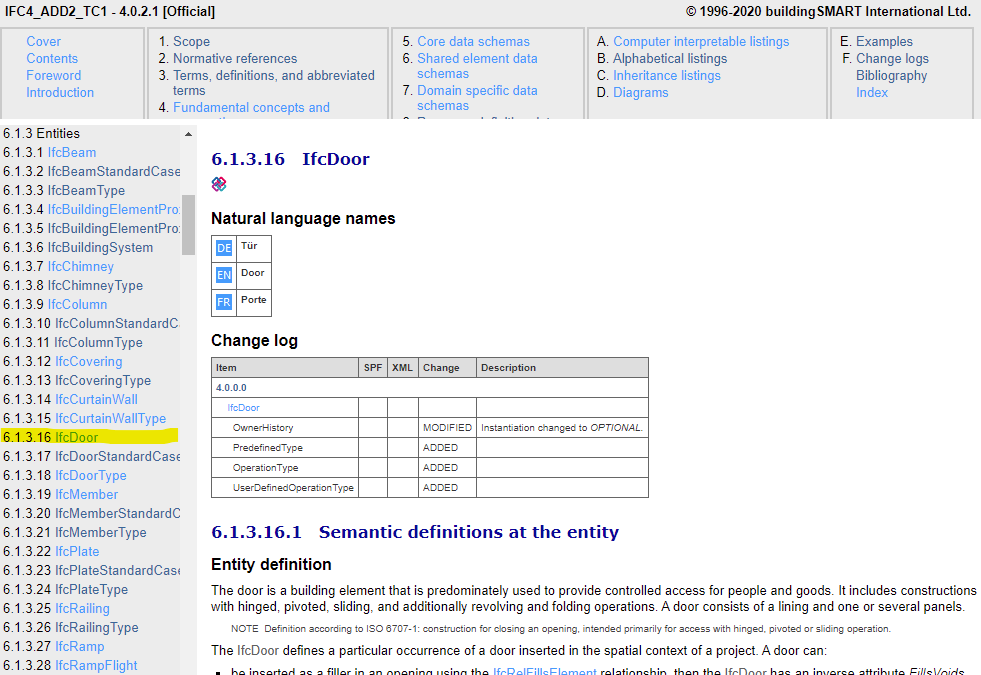
\includegraphics[width=0.8\textwidth]{IFC4 - truco - columna vertical de la izquierda}

En esa columna, la navegación es poco intuitiva y quizá demasiado ``plana''. Un buen truco para no perderse es prestar atención a los números: nos indican cuándo cambiamos de apartado, por ejemplo, en la imagen \ldots, 6.1.2.x, 6.1.3.x, 6.1.4.x, \ldots


\item aviso:
\\Navegando normalmente, haciendo clic-izdo sobre los enlaces, en la barra de direcciones se muestra solo una dirección genérica sin referencia alguna a la página que estamos viendo.
\\Navegando con clic-dcho`Abrir ventana en nueva pestaña' se muestra la dirección de la página correspondiente, pero se pierde la columna de la izquierda. 

Si queremos pasar a alguien el enlace a una página concreta, y que esta se le abra con la columna de la izquierda activa: utilizar el enlace `Link to this page' que se encuentra al final de todas las páginas.

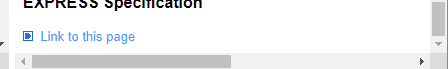
\includegraphics[scale=0.6]{IFC4 - truco - link to this page}

\item En muchas páginas, sus apartados internos se pueden colapsar/desplegar clicando sobre el título del apartado. Pero estos títulos no muestran ningún tipo de indicación del estado del apartado. 
\\aviso: Al no distinguirse visualmente si está colapsado o no, es posible que pasemos por alto información presente en alguno de los apartados. (Por ejemplo `Concept inheritance' al fondo de la página, suele venir siempre colapsado por defecto.)

\item La búsqueda del navegador ([\hspace{0,05cm}{\footnotesize CTRL}\hspace{0,05cm}]\hspace{0,1cm}[\hspace{0,05cm}F\hspace{0,05cm}]) es muy útil, sobre todo en los apartados con listados generales: `Index', `Alphabetical listings', `Inheritance listings', \ldots

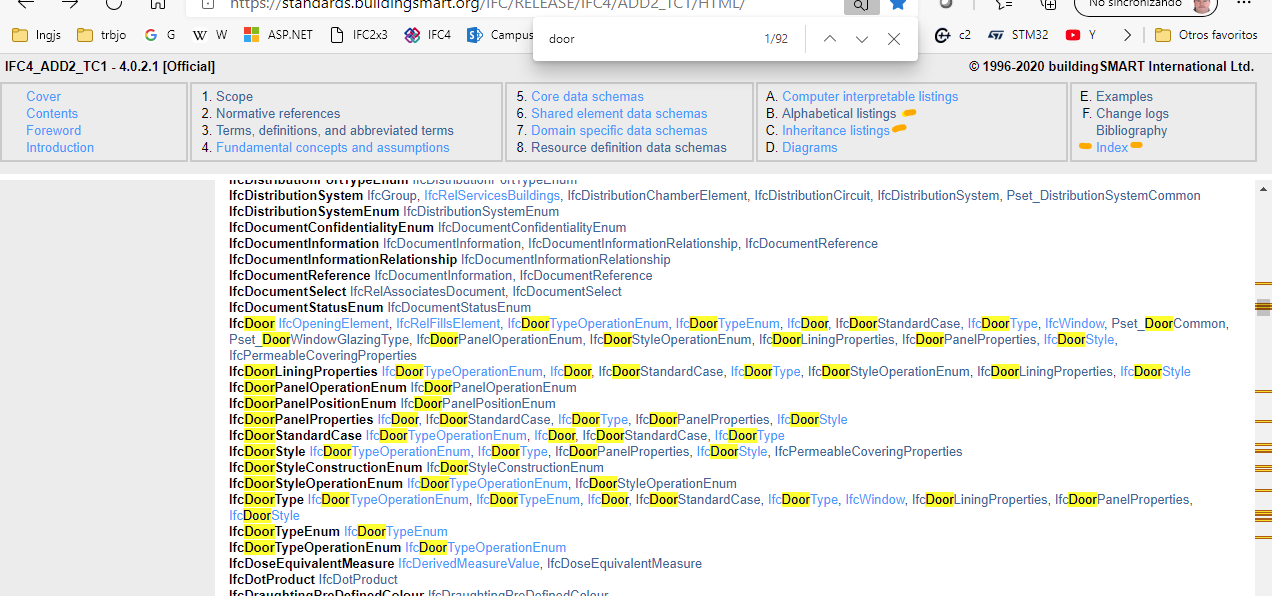
\includegraphics[width=\textwidth]{IFC4 - truco - usar la busqueda ctrl-f}

\end{itemize}


\vspace{1cm}
\textbf{Repaso general de los principales apartados:}

\vspace{0.5cm}
Los primeros apartados:
\begin{itemize}
\item 1. Scope
\item 2. Normative references
\item 3. Terms, definitions, and abbreviated terms
\item y los introductorios de `Foreword' e `Introduction'.
\end{itemize}
son para situar el terreno, explicando el propósito del estándar y su alcance.

\vspace{0.5cm}
El apartado:
\begin{itemize}
\item 4. Fundamental concepts and assumptions
\end{itemize}
permite explorar el esquema por grupos funcionales de conceptos:
\\ 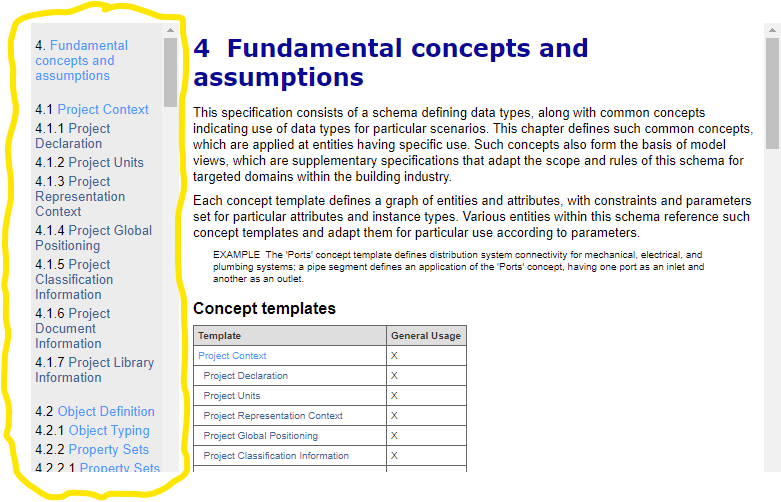
\includegraphics[width=0.9\textwidth]{IFC4 - apartado 4 - Fundamental concepts and assumptions}

\vspace{0.5cm}
Las distintas capas (layers) del esquema, están en los apartados:
\begin{itemize}
\item 5. Core data schemas $\rightarrow$ las clases (muchas de ellas abstractas) que forman el armazón troncal del esquema.
\item 6. Shared element data schemas $\rightarrow$ las clases que pueden ser de varias disciplinas, por ejemplo  edificios (arquitectura y estructuras), instalaciones (MEP).
\item 7. Domain specific data schemas $\rightarrow$ las clases que son exclusivas de una sola disciplina concreta, por ejemplo: arquitectura, electricidad, aire acondicionado, fontaneria, estructura, \ldots
\item 8. Resource definition data schemas $\rightarrow$ las clases relativas a los procesos constructivos: actores, tareas, costos, tareas, planificación, fechas,\ldots 
\end{itemize}

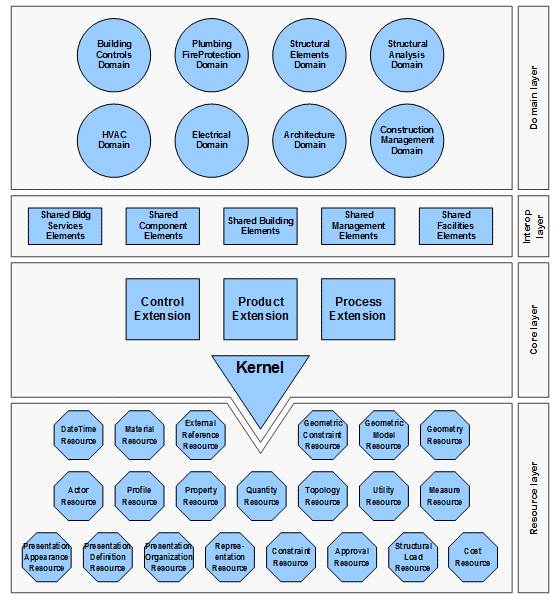
\includegraphics[width=\textwidth]{IFC4_layered_architecture}

\newpage
\vspace{0.5cm}
Para localizar con rapidez una clase concreta, son muy útiles los apartados:
\begin{itemize}

\item B. Alphabetical listings $\rightarrow$ según distintos idiomas \footnote{Por ahora: completo en inglés ; parcial en alemán (DE) y francés (FR) ; y bastante incompletos en japones, tatar y chino}.
\\ 

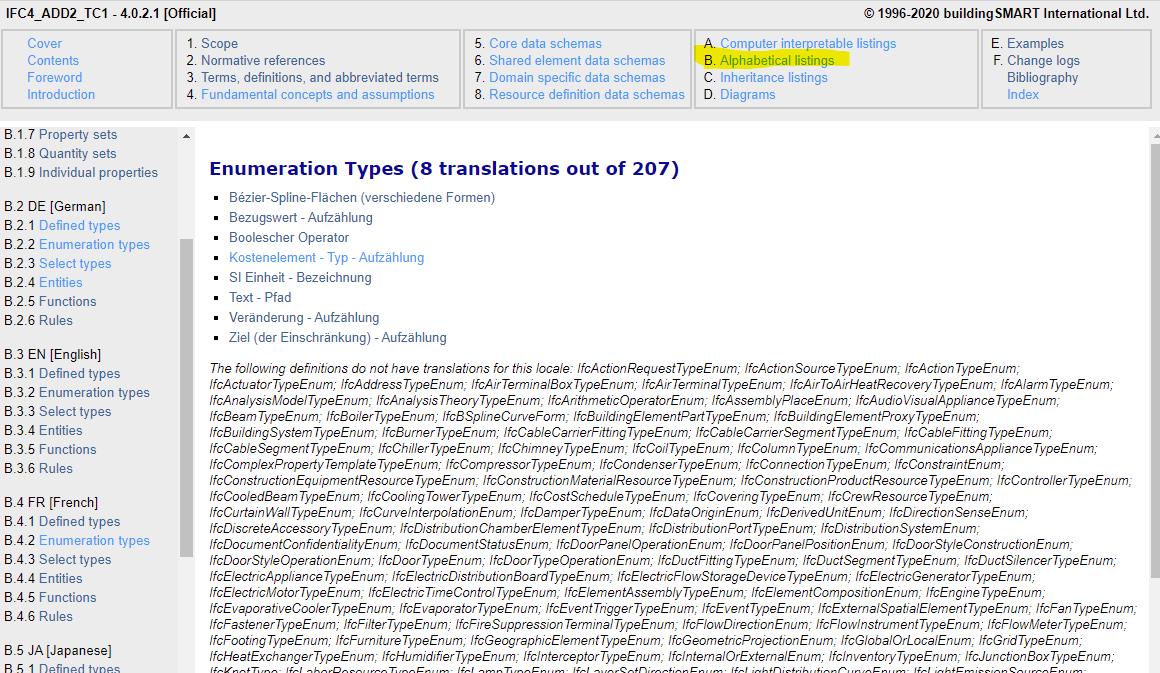
\includegraphics[width=\textwidth]{IFC4 - B - Alphabetical listings}

\item C. Inheritance listings $\rightarrow$ según qué clase deriva de cual.

Mostrando las clases en estructura arbórea:
\\ 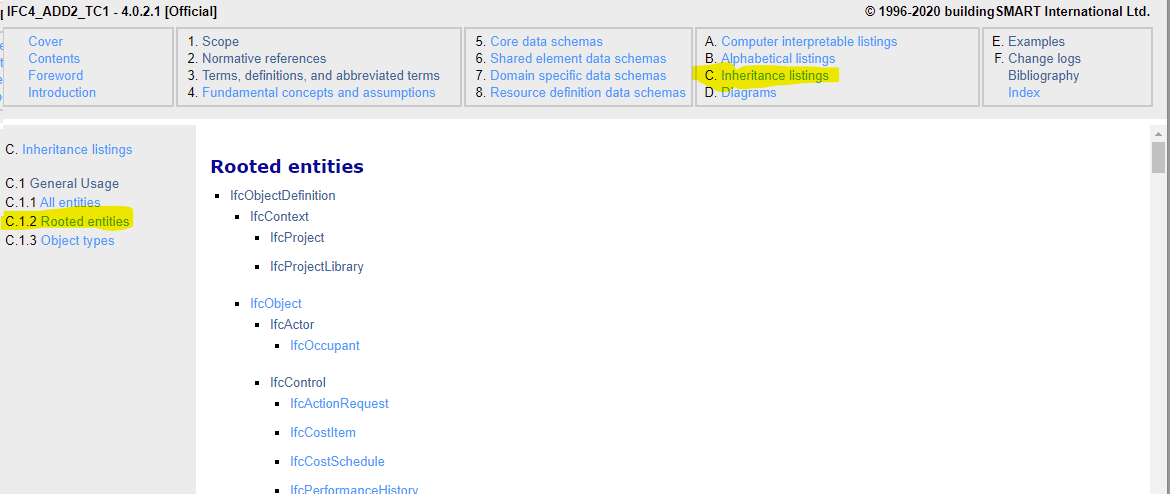
\includegraphics[width=\textwidth]{IFC4 - C - Inheritance listings - Rooted entities}

Mostrando las enumeraciones de tipo de cada clase (muy útil para verificar rápidamente si una clase es lo que pensamos que es o no):
\\ 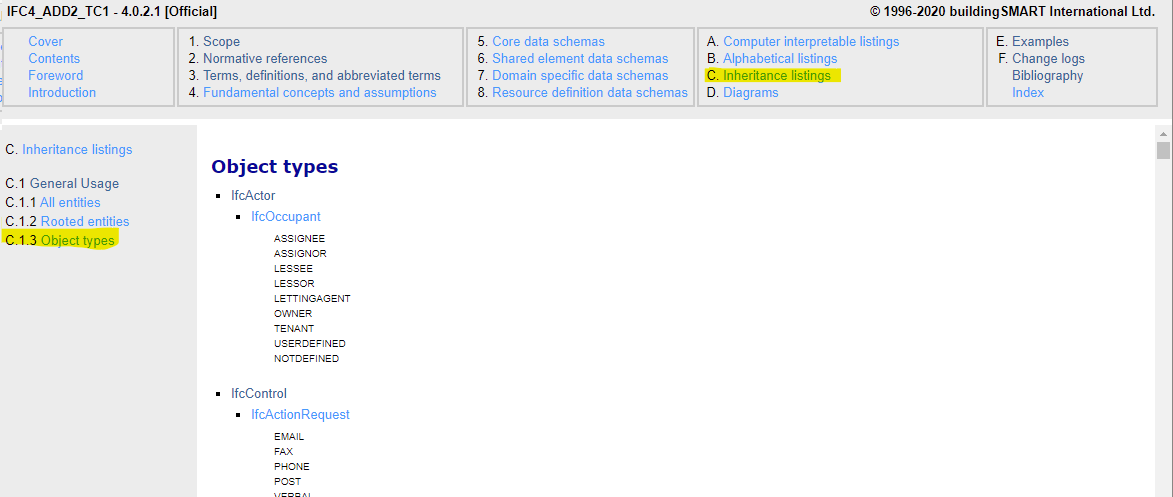
\includegraphics[width=0.9\textwidth]{IFC4 - C - Inheritance listings - Object types}

\item Index$\rightarrow$ listando todas las clases, en orden alfabético.
\\ 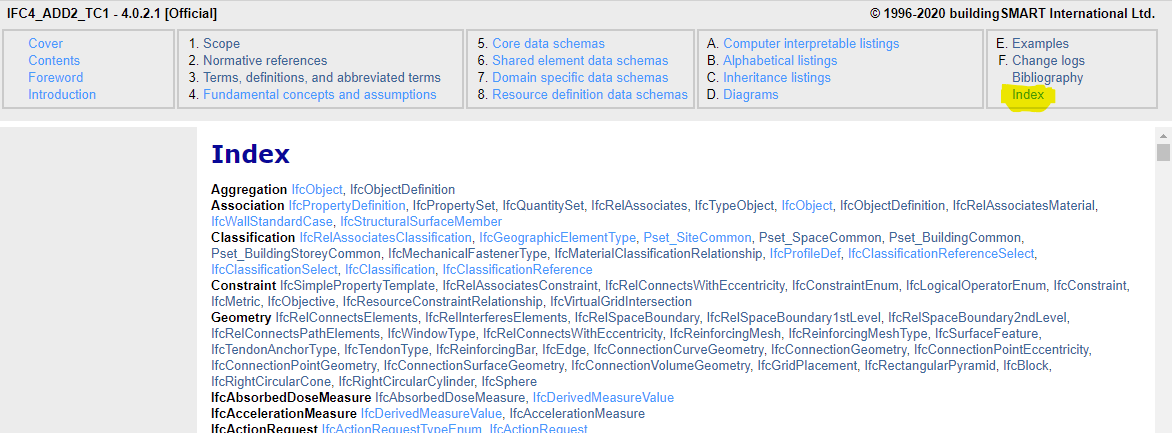
\includegraphics[width=\textwidth]{IFC4 - Index}

\end{itemize}
Truco: en todos estos apartados es muy útil la búsqueda del navegador [\hspace{0,05cm}{\footnotesize CTRL}\hspace{0,05cm}]\hspace{0,1cm}[\hspace{0,05cm}F\hspace{0,05cm}]

\vspace{0.5cm}
El apartado:
\begin{itemize}
\item D. Diagrams
\end{itemize}

En su parte D.1 Schema Diagrams contiene los diagramas EXPRESS-G de las clases principales.
\\ 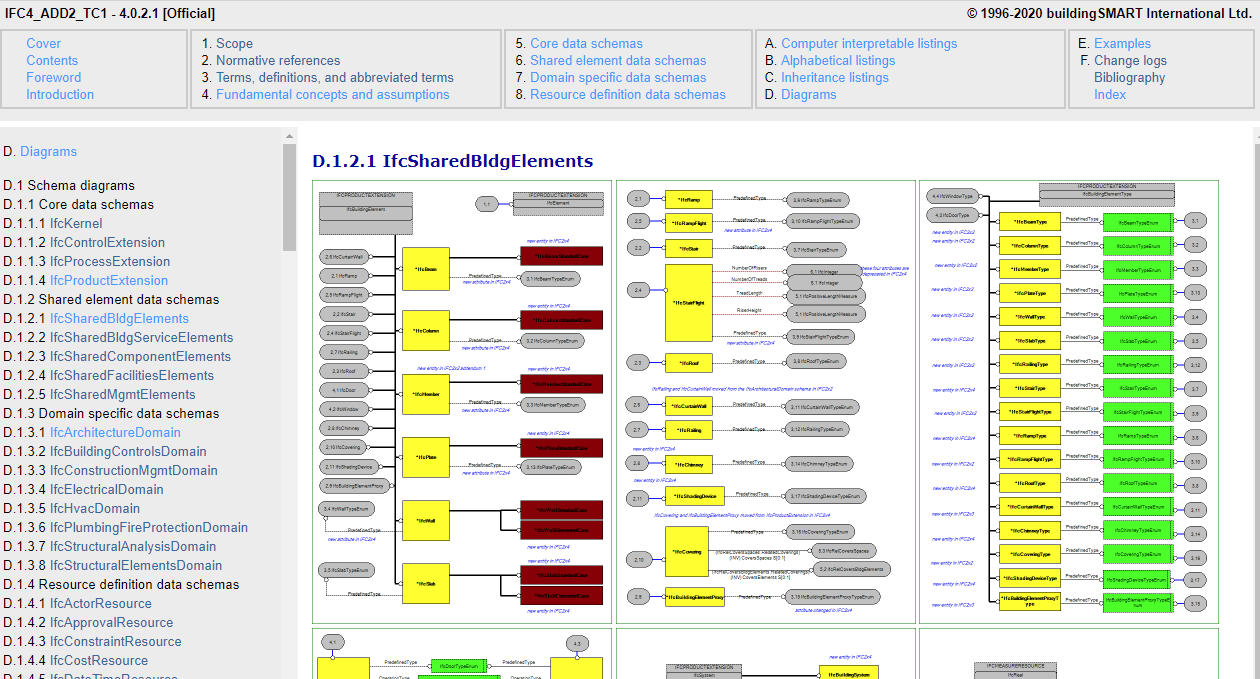
\includegraphics[width=\textwidth]{IFC4 - D - Schema Diagrams}


En su parte D.2 Instance Diagrams puede parecer un poco ``intimidante'' al principio.
\\ 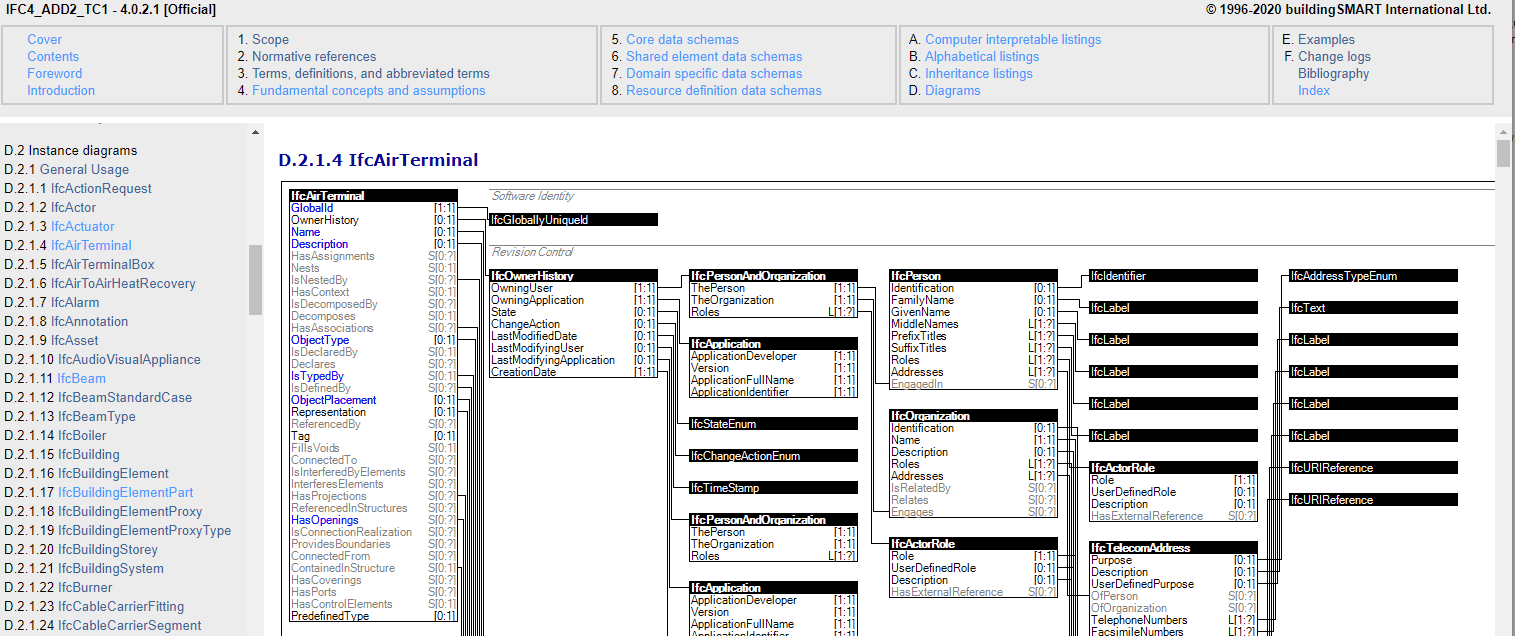
\includegraphics[width=\textwidth]{IFC4 - D - Instance Diagrams}

Pero tomando el tiempo necesario para seguir la `maraña' de líneas, es muy útil para saber cómo se relacionan las distintas clases entre sí. Por ejemplo, para saber cómo asignar un PSet a un objeto: 
\\ 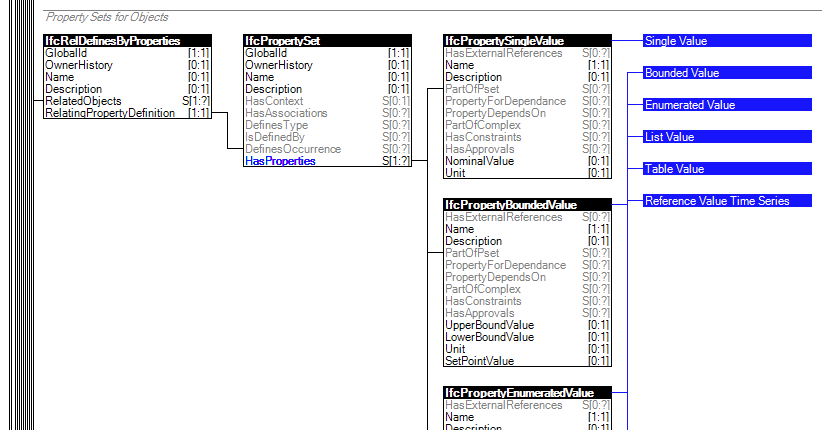
\includegraphics[width=\textwidth]{IFC4 - D - Instance Diagrams - PSet to Door}
\\truco: clicando sobre cualquiera de los textos en el diagrama, podemos ir directamente a la página de la entidad correspondiente.


\vspace{0.5cm}
El apartado:
\begin{itemize}
\item E. Examples
\end{itemize}
contiene ejemplos de aplicación de ciertos conceptos, sobre todo hay muchos ejemplos relacionados con cómo representar la geometria de objetos.
\\ 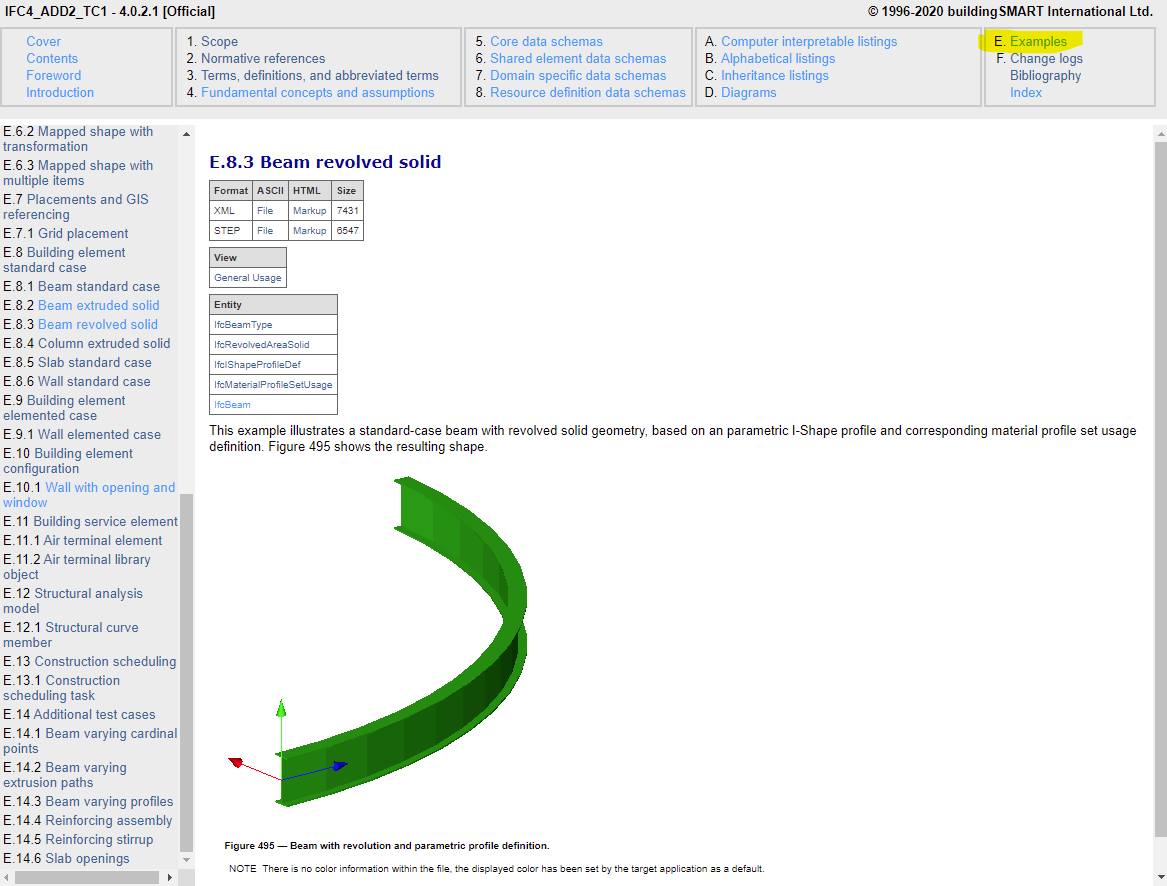
\includegraphics[width=0.5\textwidth]{IFC4 - E - Examples}

\vspace{0.5cm}
El apartado:
\begin{itemize}
\item F. Change Logs
\end{itemize}
recoge las modificaciones realizadas a las distintas clases de una versión a otra del esquema IFC.

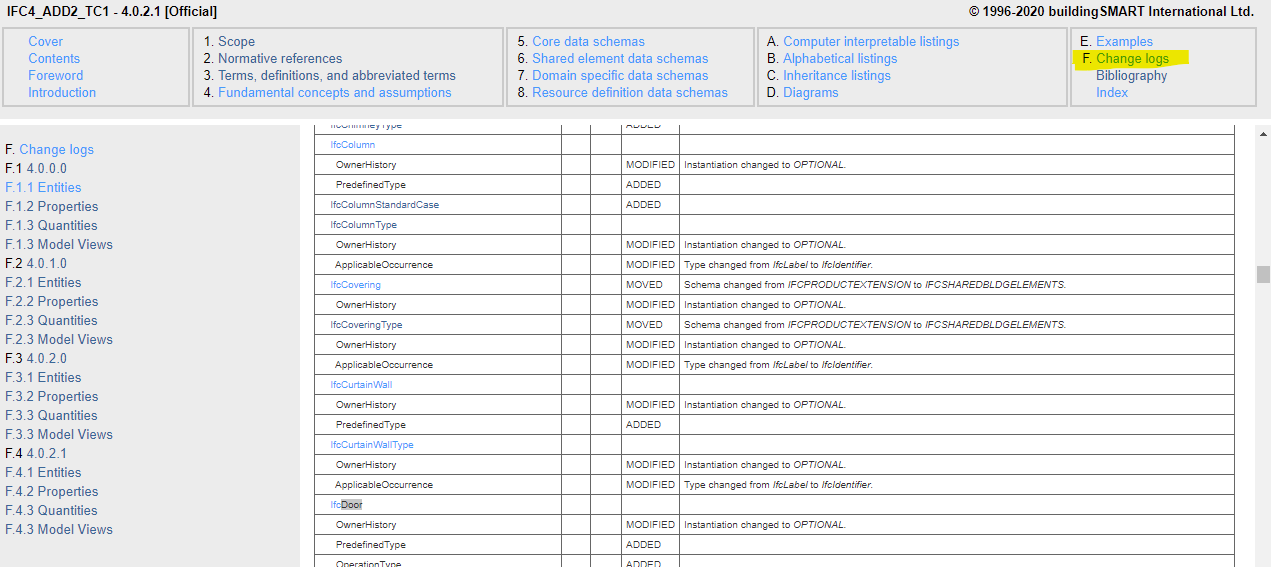
\includegraphics[width=\textwidth]{IFC4 - F - Change logs}

\vspace{0.5cm}
El apartado:
\begin{itemize}
\item A. Computer interpretable listings
\end{itemize}
da acceso a enlaces desde donde descargarse las especificaciones del esquema IFC en archivos legibles desde software, en diversos lenguajes informáticos.

\vspace{2cm}
\textbf{Principales apartados en cada página de cada entidad}

Aviso importante:
\\Estos apartados internos se pueden colapsar/desplegar clicando sobre su título. Pero los títulos no muestran ninguna indicación del estado del apartado. 
\\Al no distinguirse visualmente si está colapsado o no, es posible que pasemos por alto información presente en alguno de los apartados. (Por ejemplo `Concept inheritance' al fondo de la página, suele venir siempre colapsado por defecto.)

\begin{description}

\item[Change Log] Recoge los cambios que se han sucedido en la entidad a lo largo de las distintas versiones. Es útil para saber cuándo se introdujo por primera vez. Y suele ser importante también para saber si ha sido ``deprecated'' (a no seguir utilizando en desarrollos nuevos), junto con la entidad que la reemplaza en ese caso (la que se ha de usar).

\item[Entity definition] Explica qué es la entidad y para qué usos se ha diseñado.

\item[Attribute definitions] Una tabla con todos los atributos propios de la entidad, detallando para cada uno de ellos:
\begin{itemize}
\item El tipo de valor que admite:  IfcXxxxxxxxx
\item La cardinalidad (cuántos valores admite; importante sobre todo en las entidades que representan relaciones, ya que indica cuántas entidades pueden participar en cada uno de los dos sentidos de la relación). 
\end{itemize}

\item[Entity inheritance] Un diagrama con la jerarquia de herencias, indicando las entidades ``madre'' de las que esta deriva.

\item[Attribute inheritance] Una tabla consolidada con todos los atributos que la entidad puede tener (tanto heredados como propios).

\item[Concept usage] Aclaraciones acerca de cómo utilizar la entidad. Según la complejidad de esta, puede tener más o menos apartados:
\begin{itemize}
\item Attributes
\item Object Typing
\item Property Sets
\item Quantity Sets
\item Material Constituent Set
\item Product Local Placement
\item Profile 3D Geometry
\item Spatial Containment
\item etc.
\end{itemize}

\item[Concept inheritance] Detalle consolidado de los usos que se aplican a esta entidad y de dónde los recibe (hereda).

\item[Formal representations] La definición propiamente dicha de la entidad, expresada en lenguajes informáticos, aptos para ser procesados por máquinas.
\begin{itemize}
\item mvdXML Specification
\item XML Specification 
\item EXPRESS Specification
\end{itemize}

\end{description}



\vspace{4cm}
\subsubsection{Especificaciones del esquema IFC en su versión 2x3 (IFC2X3 TC1)}

\includegraphics[width=\textwidth]{IFC2X3 - Portada}

\url{https://standards.buildingsmart.org/IFC/RELEASE/IFC2x3/TC1/HTML/}





\newpage
\section{Comprensión (IV) a través de software de visualización y revisión de modelos de información basados en IFC Schema}

\subsection{ifcDOC, una herramienta para visualizar el propio esquema IFC}
\url{https://github.com/buildingSMART/IfcDoc}

nota: Para utilizarla, se puede descargar el ejecutable desde el apartado `Releases'. No necesita instalación, se arranca ejecutando directamente el archivo IfcDoc.exe de la carpeta donde se descomprima el .zip descargado.
\\ 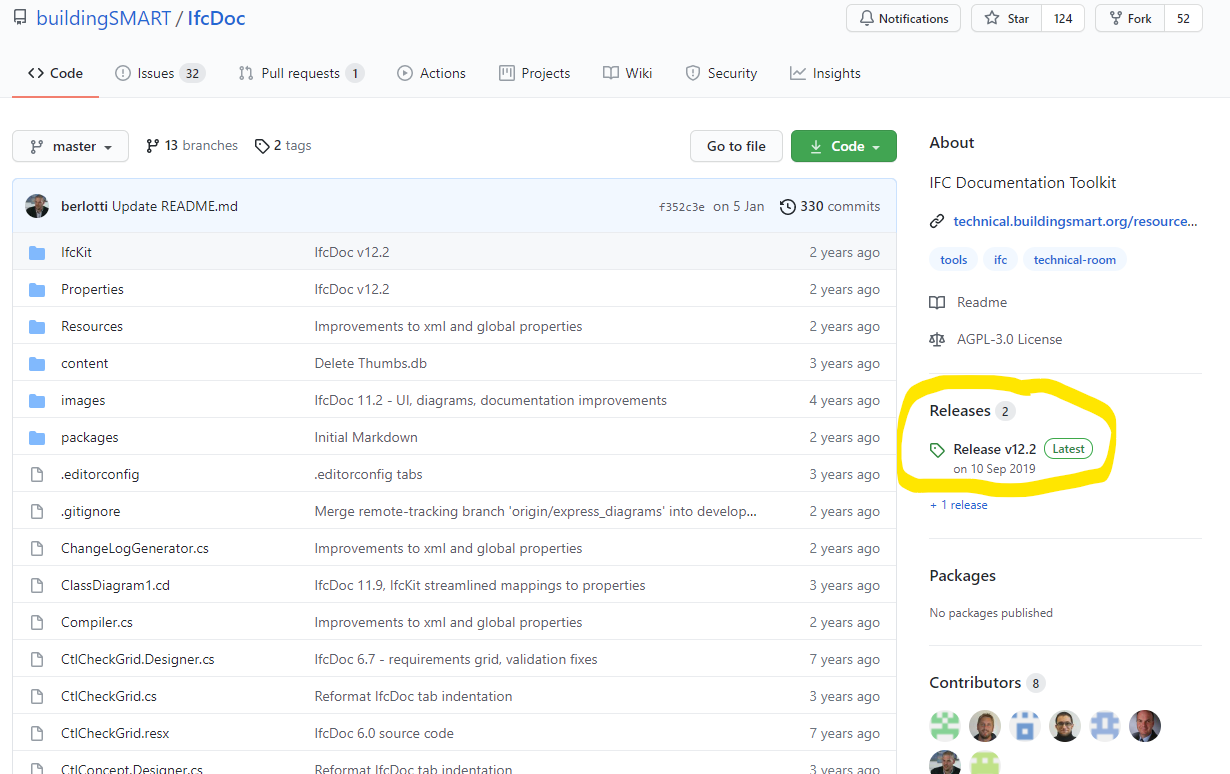
\includegraphics[width=\textwidth]{ifcDOC en github}
\\nota: Los archivos *.ifcdoc que necesita para cargar las especificaciones de cada versión del esquema IFC, se pueden descargar desde ???

\vspace{1cm}

ifcDOC es una herramienta que se preparó para compilar y formatear la documentación IFC en distintos formatos.

Hace unos años, permitía elaborar nuestro propio subconjunto del esquema (un MVD) y exportarlo a un archivo mvdXML para utilizarlo, por ejemplo, en softwares de validación de modelos. Pero la versión actual no tiene esa funcionalidad.
\\ \url{https://github.com/buildingSMART/IfcDoc/wiki/IfcDoc-User-Guide}
\\ \url{https://forums.buildingsmart.org/c/developers/ifcdoc-tool/52}

En estos momentos el desarrollo del esquema IFC se está moviendo desde el lenguaje EXPRESS a UML\ldots en un futuro\ldots ¿continuará el desarrollo de ifcDOC en esa otra línea?

De todas formas, tal y como está ahora, ifcDOC permite visualizar las especificaciones del esquema IFC. Con una forma más cómoda de navegar que en la web, ya que los árboles son desplegables. Pero con un renderizado de gráficos y textos bastante peor que en la web.

El contenido mostrado es prácticamente el mismo que se muestra en la web.
\\ \url{https://technical.buildingsmart.org/standards/ifc/ifc-schema-specifications/}. 



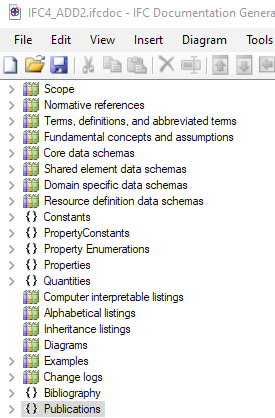
\includegraphics[scale=0.9]{ifcDOC vs web - contenido ifcDOC}

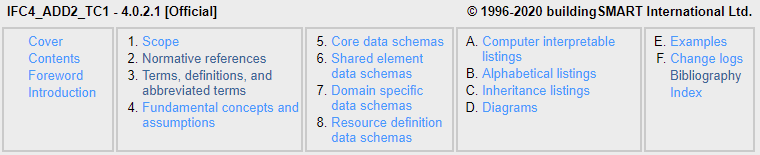
\includegraphics[width=1.1\textwidth]{ifcDOC vs web - contenido web}
\\nota: en la web nos hemos de guiar por los números de sección a la hora de navegar.
\\nota: en la web, los esquemas EXPRESS-G están al fondo de la página de cada entidad (cliclar sobre `EXPRESS Specification' para desplegar ese apartado)
\begin{flushright}
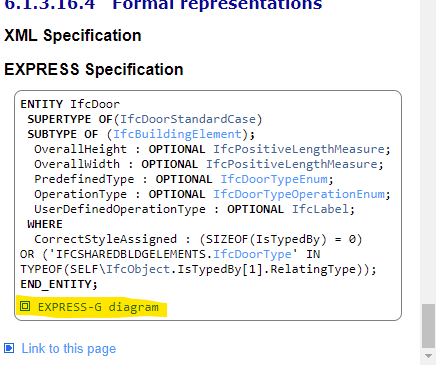
\includegraphics[scale=0.4]{ifcDOC vs web - diagrama esta en el fondo}
\hspace{1cm}
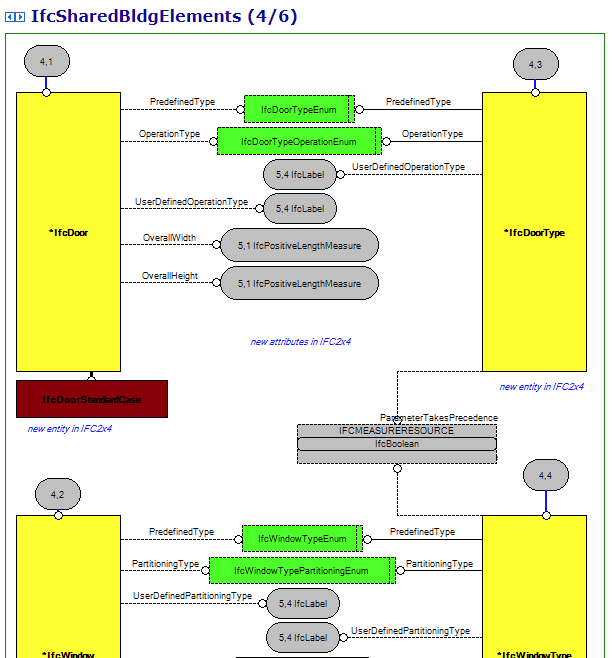
\includegraphics[scale=0.3]{ifcDOC vs web - diagrama}

\end{flushright}

\vspace{1cm}

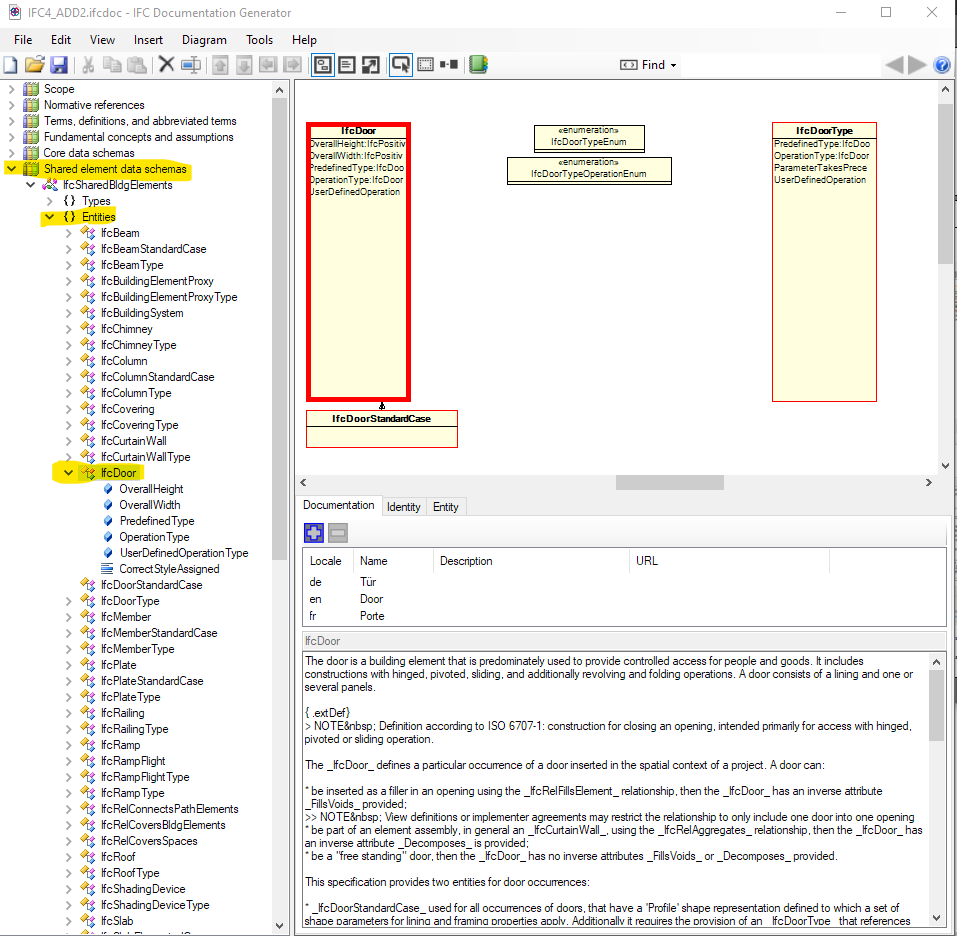
\includegraphics[width=\textwidth]{ifcDOC vs web - pantallazo ifcDOC}

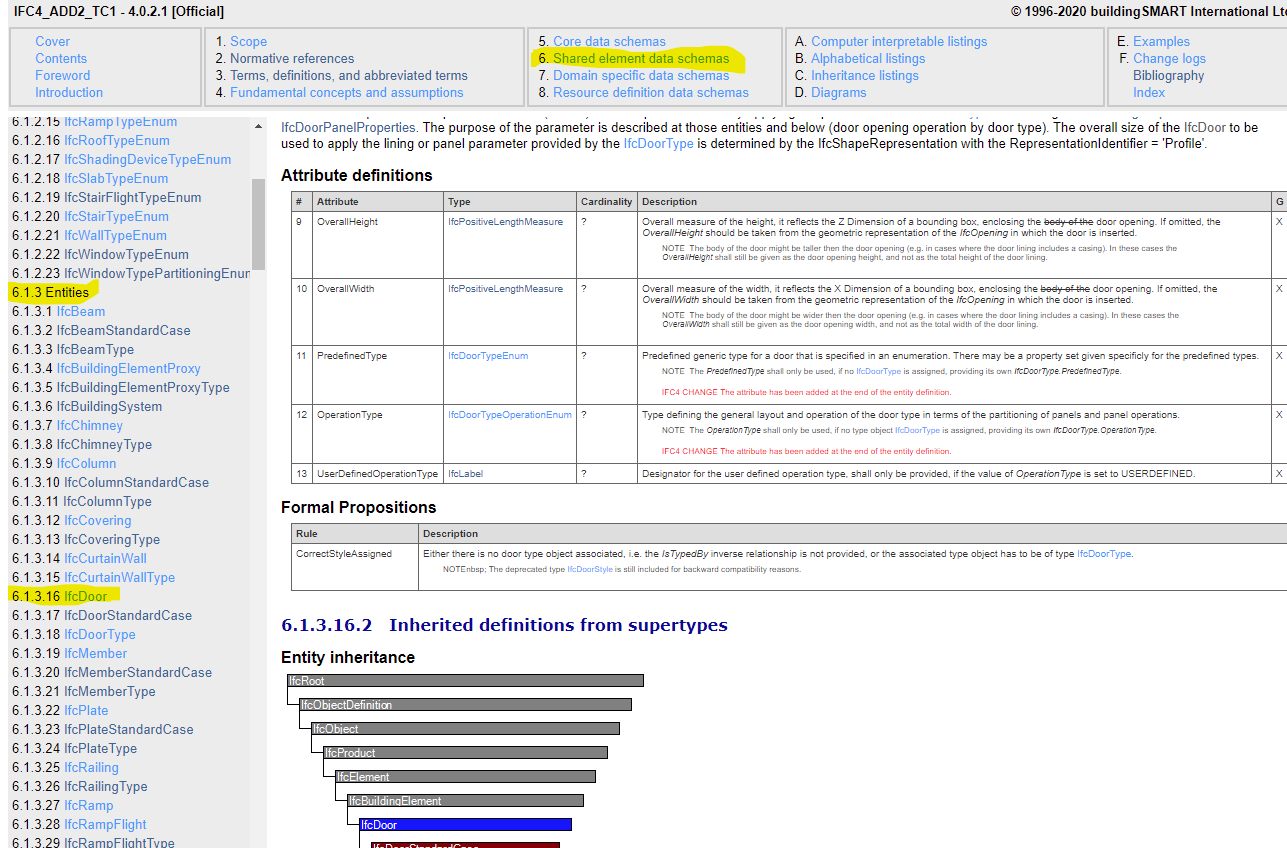
\includegraphics[width=\textwidth]{ifcDOC vs web - pantallazo web}



\subsection{Un repaso a los diversos softwares de visualización IFC que hay en el mercado}

nota: Cada herramienta tiene sus peculiaridades. Un mismo modelo IFC se ve de manera algo distinta en cada una de ellas.

\begin{description}

\item[Geometry Gym]
\url{https://geometrygym.wordpress.com/}
\\Es un visualizador de texto, que muestra directamente el código STEP del modelo IFC. Pero con funcionalidades que lo reorganizan y lo muestran en forma de árbol desplegable para facilitar la navegación.

\item[IFC File Analyzer]
\url{https://www.nist.gov/services-resources/software/ifc-file-analyzer}
\\Transforma un modelo IFC en una hoja de cálculo.
\\nota: si se activan todas sus opciones, sobre todo la de incluir relaciones inversas, la conversión puede llevar bastante tiempo\ldots tener paciencia.

\item[Xbim Xplorer]
\url{https://docs.xbim.net/downloads/xbimxplorer.html}
\\Es un programa que se construyó como demostrador de la biblioteca de programación Xbim Toolkit (https://docs.xbim.net/) (https://github.com/xBimTeam) para .NET
\\Permite cargar varios modelos IFC para verlos de forma federada.
\\Admite ampliar sus capacidades por medio de plugins. Por ejemplo, tiene uno que permite verificar el modelo contra un MVD concreto ({\footnotesize usando la descripción de este en un archivo mvdXML})
\\aviso: tiene tendencia a cascar con modelos grandes.

\item[ODA OpenIFC viewer]
\url{https://openifcviewer.com/}

\item[DDS-CAD]
\url{https://www.dds-cad.net/downloads/dds-cad-viewer/}

\item[BIMData viewer]
\url{https://bimdata.io/visionneuse-bim/}

\item[BIMvision]
\url{https://bimvision.eu/es/}
\\Es un visor gratuito. Pero algunos de sus plugins (\url{https://bimvision.eu/es/plugins-es/}) (por ejemplo el que permite federar varios modelos) son de pago.
\\Permite ver el modelo IFC en forma de árbol según códigos de clasificación, si es que el modelo trae asociado algún esquema de clasificación externo.

\item[UsBIM.viewer+]
\url{https://www.accasoftware.com/es/visor-ifc}
\\Permite editar el modelo para hacerle ajustes manuales en propiedades, en clasificación de entidades o incluso en el posicionamiento geométrico de entidades.
\\Permite importar archivos XML (formato Archicad) con sistemas de clasificación, para facilitar la (re)clasificación de entidades.


\item[BIM Collab ZOOM]
\url{https://support.bimcollab.com/en/Support/Support/Downloads}
\\Esta herramienta y sus plugins tienen versiones gratuitas (con funcionalidad limitada) y de pago (\url{https://www.bimcollab.com/en/products/bimcollab-zoom}).
\\Una de sus funcionalidades de pago son las ``smart views''. Permiten controlar la visualización en base a conjuntos de reglas o filtros que se definan según las necesidades de revisión/verificación que se tengan. Por ejemplo, permiten mostrar en distintos colores entidades con distintos valores en unos ciertos parámetros. (\url{https://www.bimcollab.com/en/products/bimcollab-zoom/smart-views})
\\Otra de esas funcionalidades son las ``lists''. Permiten extraer subconjuntos de datos de los modelos, para facilitar la focalización en aspectos concretos o para mostrarlos en otros programas externos. (\url{https://www.bimcollab.com/en/products/bimcollab-zoom/lists}
\\Otra es la posibilidad de compartir vistas o listas en la nube. (\url{https://www.bimcollab.com/en/products/bimcollab-cloud}) 

\item[Solibri Anywhere]
\url{https://www.solibri.com/solibri-anywhere}
\\Tiene otras versiones de pago, con funcionalidades adicionales:
\\ \url{https://www.solibri.com/solibri-office#features}
\\ \url{https://www.solibri.com/solibri-site}
\\ \url{https://www.solibri.com/solibri-enterprise}

\item[SimpleBIM]
\url{https://simplebim.com/features/}
\\Es una herramienta de pago.
\\Permite editar modelos IFC y automatizar todo tipo de procesos de validación o transformación de los mismos.

\end{description}




\newpage
\section{Introducción al proyecto IFC5 Next Gen y debate en relación al futuro de los intercambios de información en un marco openBIM en los disintos ámbitos del ciclo de vida de los activos}

Dentro del proyecto NextGen IFC5, se avecinan cambios bastante profundos:

\begin{itemize}

\item En la definición del esquema IFC, cambiar el lenguaje EXPRESS por diagramas \textbf{UML}.

\item En los archivos e intercambios de información, cambiar el lenguaje STEP por \textbf{XML} o \textbf{JSON} o \textbf{RDF/OWL} (Linked Data).

\item Cambiar desde un uso orientado a intercambio de archivos, hacia un uso orientado a servicios web (\textbf{API}).

\item Evolucionar los conceptos de IDM (Information Delivery Manual) y MVD (Model View Definition) hacia unas especificaciones más flexibles y que sean legibles desde software: \textbf{IDS} (Information Delivery Specification) 

\end{itemize}

\url{https://www.buildingsmart.org/about/technical-roadmap/}

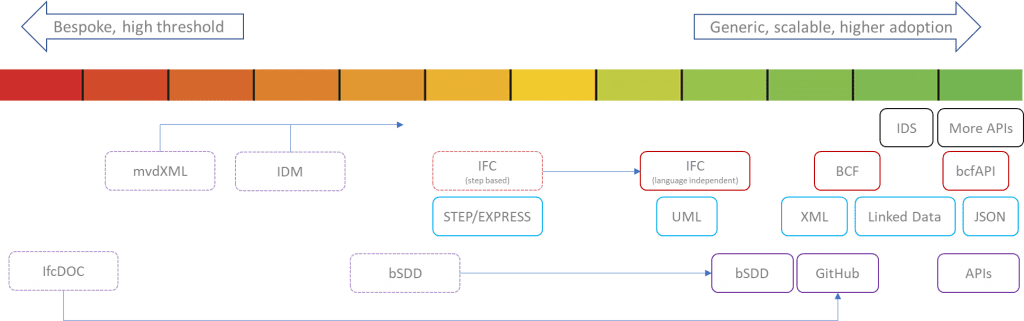
\includegraphics[width=\textwidth]{NextGen IFC5 roadmap}

También se están considerando otros cambios tales como:
\begin{itemize}
\item Usar gltF como representación geométrica básica estandarizada.
\item Usar UTF8 como representación para codificar caracteres.
\item Usar cifras hexadecimales tal cual, en lugar de usar codificación Base64 para ahorrar cifras.
\item Simplificar definiciones, evitando duplicidades y cuidando la coherencia general en todo el esquema IFC.
\item Potenciar la modularidad, para facilitar cambios y evoluciones ágiles en los distintos aspectos del esquema IFC.
\end{itemize}

{\tiny Para más detalles, descargar el PDF desde los enlaces previstos para tal efecto en la página web de buildintSMART acerca del technical-roadmap. En este momento \url{https://buildingsmart-1xbd3ajdayi.netdna-ssl.com/wp-content/uploads/2020/09/20200430_buildingSMART_Technical_Roadmap.pdf}}



\subsection{IDS (Information Delivery Specification)}

El concepto de MVD ha resultado difícil de interpretar en la práctica, complicado de implementar en los softwares y costoso de mantenerlo alineado con la evolución general en el esquema IFC.

Por eso, en IFC5 se está definiendo otro sistema, el IDS, que permita configurar, a los propios usuarios y de forma flexible:
\begin{itemize}
\item los requisitos de intercambio de información
\item los módulos (dominios) a utilizar
\end{itemize}
La idea es que el cliente en cada proyecto pueda definir una serie de requisitos de intercambio de información. Apoyándose en las plantillas y en los UCM (Use Case Management) que se hayan definido \url{https://ucm.buildingsmart.org/} . Con total libertad y flexibilidad para utilizar las partes del esquema IFC que se precisen en cada caso.

Estos requisitos se volcarán en uno o varios IDS (Information Delivery Specification), usando un lenguaje {\footnotesize (XML)} que permita ser interpretado directamente en los softwares con los que se trabaje.
\\Con ánimo de permitir realizar exportaciones guiadas por dichos IDS. Y de permitir verificaciones automáticas de que se están cumpliendo las especificaciones en cada intercambio de información que se lleve a cabo.

nota: Este concepto de IDSs puede ayudar  a definir también PDTs (Product Data Template), por parte de los fabricantes de productos para la construcción.

nota: Este concepto de IDS se está elevando a nivel de norma, en la EN 17412-1 (Level of Information Need) y las partes que le seguiran (-2 y -3).

\subsection{bSDD, servicio de Data Dictionary}

Para facilitar que todos hablemos un idioma (lo más) común (posible). Se está preparando un repositorio donde almacenar:
\begin{itemize}
\item Traducciones a distintos idiomas de los términos relacionados con IFC.
\item Conjuntos de elementos, información, relacionados con cada entidad definida en el esquema IFC. Según prácticas habituales o estandares en distintos países o sectores de actividad.
\end{itemize}

La idea es que se pueda establecer una conexión directa a bSDD desde los propios softwares.
\\De tal forma que nos permitan realizar búsquedas tesaúricas según términos en nuestro propio idioma, filtradas según estandares de aplicación en un cierto país o sector de actividad.
\\Estas búsquedas devolverian todos los conceptos y propiedades relacionadas con el término buscado.
\\De tal forma que nos guíen en el enriquecimiento de la información en los objetos de nuestro modelo IFC.

\url{https://www.buildingsmart.org/users/services/buildingsmart-data-dictionary/}

\url{https://search.bsdd.buildingsmart.org/}

nota: Este concepto de Data Dictionary se está elevando a nivel de norma en la ISO 12006-3 (2021), Framework for Dictionaries.

\subsection{Niveles de conformidad en representación gráfica}
La representación geométrica ha resultado ser una fuente de problemas en la interoperabilidad entre los distintos softwares que trabajan con IFC.

Por eso, en IFC5 se ha puesto el foco en los datos, en la información. Garantizando que todos los softwares sean capaces de interpretarlos.

\vspace{0.3cm}
Y en cuanto a la geometría, se han definido una serie de niveles de conformidad:
\begin{description}
\item[nivel $\star$] $\rightarrow$ con geometrías básicas simplificadas.
\item[nivel $\star\star$] $\rightarrow$ con geometrías analíticas precisas.
\item[nivel $\star\star\star$] $\rightarrow$ con geometrías modificables (con historia de cómo han sido confeccionadas).
\end{description}
La idea es que todos los softwares que vayan a trabajar con IFC implementen como mínimo el nivel $\star$. Ese será el nivel universal, el nivel que todo software IFC será capaz de interpretar.
\\El nivel $\star\star$ lo podrán interpretar los softwares de nivel $\star\star$, obviamente, y también los de nivel $\star\star\star$.
\\El nivel $\star\star\star$ solo lo podrán interpretar los softwares de nivel $\star\star\star$.



\end{document}